\documentclass[12pt]{article}
\usepackage{indentfirst}
\usepackage[utf8x]{inputenc}
\usepackage[T1]{fontenc}
\usepackage[english,lithuanian]{babel}
\usepackage{array}
\usepackage{caption}
\usepackage{subcaption}
\usepackage{makecell}
\usepackage[euler]{textgreek}
\usepackage{multirow}
\usepackage{boldline}
\usepackage{floatrow}
\floatsetup[table]{capposition=top}
\usepackage{amsmath, amsthm, amssymb}
\usepackage{graphicx}
\usepackage{setspace}
\usepackage{verbatim}
\usepackage[left=3cm,top=2cm,right=1.5cm,bottom=2cm]{geometry}
\usepackage{floatrow}
\newfloatcommand{capbtabbox}{table}[][\FBwidth]
\usepackage{blindtext}
\onehalfspacing
\usepackage[hidelinks, unicode]{hyperref}
\usepackage{textcomp}
\usepackage{amsmath}
\usepackage{cleveref}
\usepackage[labelfont=bf]{caption}
\usepackage{microtype}
\usepackage{tabularx}
\captionsetup[table]{font={normalfont},format=plain,labelsep=period}
\graphicspath{{../assets/images/}}
\usepackage[table]{xcolor}
\definecolor{newGray}{rgb}{0.878, 0.878, 0.878}
\usepackage{longtable}
\usepackage{enumitem}
\definecolor{deepchampagne}{rgb}{0.98, 0.84, 0.65}
\definecolor{dartmouthgreen}{rgb}{0.09, 0.45, 0.27}
\definecolor{deepcarmine}{rgb}{0.66, 0.13, 0.24}
\definecolor{steelblue}{rgb}{0.27, 0.51, 0.71}
\usepackage{makecell}

\newcommand{\EE}{\mathbb{E}\,}
\newcommand{\ee}{{\mathrm e}}
\newcommand{\dd}{{\mathrm d}}
\newcommand{\RR}{\mathbb{R}}

\begin{document}
\selectlanguage{lithuanian}

\begin{titlepage}
\vskip 20pt
\begin{center}
\includegraphics[scale=1.4]{KTU.png}
\end{center}

%%%%%%%%%%%%%%%%%%%%%%%
% TITULINIS PUSLAPIS
%%%%%%%%%%%%%%%%%%%%%%%

\vskip 20pt
\centerline{\bf \large \textbf{Kauno technologijos universitetas}}
\bigskip
\centerline{\large {Informatikos fakultetas}}
\bigskip

\vskip 90pt
\begin{center}
    {\bf \LARGE Modulis „Tiriamasis projektas 2“}
    \vskip 10pt
    {\bf \Large Projektas: „Savarankiškos suverenios pseudonimizuotos tapatybės 
    valdymo sistema“}
    \vskip 15pt
    {\large Reikalavimų specifikavimas}
\end{center}

\vskip 40pt

\hskip 200pt {\bf \large IFM 4/2 gr. Danielė Stasiūnaitė}
\vskip 1pt
\hskip 200pt {\large Studentė}
\vskip 7pt
\hskip 200pt {\bf \large Doc. Mindaugas Vasiljevas}
\vskip 1pt
\hskip 200pt {\large Projekto vadovas}
\vskip 7pt
\hskip 200pt {\bf \large Doc. dr. Eglė Butkevičiūtė}
\vskip 1pt
\hskip 200pt {\large Dėstytoja}

\bigskip

\vskip 100pt
\centerline{\large \textbf{Kaunas, 2025}}
\newpage
\end{titlepage}

\selectlanguage{lithuanian}

%%%%%%%%%%%%%%%%%%%%%
% TURINIO PUSLAPIS
%%%%%%%%%%%%%%%%%%%%%

\tableofcontents
\newpage

\section{Sistemos paskirtis}
\subsection{Projekto kūrimo pagrindas (pagrindimas)}
Skaitmeniniame amžiuje, kai asmens duomenys tampa viena svarbiausių vertybių,
privatumo užtikrinimas ir efektyvus tapatybės valdymas yra pagrindiniai
iššūkiai, su kuriais turi susidurti ne tik privatūs asmenys, bet ir įvairios
organizacijos. Sparčiai augantys informacijos srautai, elektroninių paslaugų
plėtra bei kitų paslaugų, reikalaujančių naudotojų autentifikacijos, vystymas
lėmė inovatyvių technologinių sprendimų - blokų grandinės pritaikymo, 
realizuojant decentralizuotos asmens tapatybės valdymo modelį - kūrimą.
Pastaruoju sprendimu siekiama užtikrinti asmens duomenų saugumą bei visapusišką
duomenų kontrolę, kuri atliekama paties naudotojo.

Šiuo metu egzistuojančios asmens tapatybės valdymo sistemos, pavyzdžiui,
centralizuotos ar federacinės, dažnai susiduria su privatumo, duomenų apsaugos
ir patogumo iššūkiais. Centralizuotos sistemos yra itin jautrios saugumo
pažeidimams, o federacinės sistemos dažnai riboja naudotojo autonomiją. Šie
trūkumai skatina naujų sprendimų kūrimo poreikį, orientuotą į naudotojo teisių
ir privatumo stiprinimą.

Šis projektas skirtas sukurti savarankiškos suverenios pseudonimizuotos
tapatybės valdymo sistemą, kuri leistų naudotojams
ne tik valdyti asmeninę informaciją ir dalinimąsi ja, bet ir užtikrintų, kad
asmeniniai duomenys negalėtų būti lengvai susieti su naudotoju, kurį šie
duomenys apibūdina. Šie tikslai bus pasiekti, pritaikius decentralizuotos
tapatybės valdymo modelį, kuris grindžiamas blokų grandinės technologija,
duomenų šifravimo bei pseudonimizavimo metodikomis.

\subsection{Sistemos tikslai (paskirtis)}
Sistemos kūrimo projektu siekiama įgyvendinti šiuos tikslus:
\begin{itemize}
    \item 1
    \item 2
    \item 3
    \item 4
    \item 5
\end{itemize}

\section{Užsakovai, pirkėjai ir kiti sistema suinteresuoti asmenys}
\subsection{Užsakovas}
Sistemos kūrimo projektą užsako darbo vadovas Mindaugas Vasiljevas. Užsakovo
rolės projekte apima sistemos finansavimo, reikalavimų sistemai rinkimo ir
teikimo bei konsultacijų, susijusių su dalykine sritimi, teikimą.
Darbo vadovo kontaktiniai duomenys:

\begin{table}[htb!]
    \captionsetup{justification=centering}
    \caption{\small\textbf{Panaudojimo atvejo specifikacija Nr.2.}}
    \begin{tabular}{|m{6cm}|m{11cm}|}
        \hline
        \raggedleft \textbf{\cellcolor{deepchampagne}Mobilusis telefonas:} &
        +37066428763. \\
        \hline
        \raggedleft \textbf{\cellcolor{deepchampagne}El. pašto adresas} &
        mindaugas.vasiljevas@ktu.lt. \\
        \hline
        \raggedleft \textbf{\cellcolor{deepchampagne}Adresas} & 
        XI rūmai 3C2b korpusas. \\
        \hline
        \raggedleft \textbf{\cellcolor{deepchampagne}Informacijos galima teirautis}
        & I - V; 10:00 - 17:00. \\
        \hline
    \end{tabular}
    \label{table:kontaktiniai_duomenys}
\end{table}

\subsection{Pirkėjas}
Sistemos pirkėjas sutampa su sistemos užsakovu.

\subsection{Naudotojai}
Žemiau yra pateikiami potencialių sistemos naudotojų - pacientų, gydytojų ir
tyrėjų - aprašymai kartu su šių naudotojų charakteristikomis.

\subsubsection*{Pacientai}
\label{sec:N1}
\begin{table}[htb!]
    \captionsetup{justification=centering}
    \vskip -10pt
    \begin{tabular}{|m{4cm}|m{12cm}|}
        \hline
        \raggedleft \textbf{\cellcolor{deepchampagne}Funkcijos} &
        Valdyti savo asmeninių genetinių duomenų prieinamumą kitoms naudotojų
        grupėms; esant poreikiui, įkelti genetinius duomenis; peržiūrėti
        analizių, atliktų su genetiniais duomenimis, rezultatus. \\
        \hline
        \raggedleft \textbf{\cellcolor{deepchampagne}Patirtis dalykinėje
        srityje} & Žema. \\
        \hline
        \raggedleft \textbf{\cellcolor{deepchampagne}Patirtis IT srityje} &
        Žema. \\
        \hline
        \raggedleft \textbf{\cellcolor{deepchampagne}Papildomos
        charakteristikos} &
        Sistema besinaudojančius
        pacientus sieja kalba (lietuvių kalba) ir interesai (valdyti savo
        asmeninius genetinius duomenis, kurie gali būti panaudoti, net tik
        atliekant asmens genetinius tyrimus, bet ir moksliniais tikslais). \\
        \hline
        \raggedleft \textbf{\cellcolor{deepchampagne}Prioritetas} & Aukštas. \\
        \hline
    \end{tabular}
\end{table}

\newpage

\subsubsection*{Gydytojai - genetikai}
\label{sec:N2}
\begin{table}[htb!]
    \captionsetup{justification=centering}
    \vskip -10pt
    \begin{tabular}{|m{4cm}|m{12cm}|}
        \hline
        \raggedleft \textbf{\cellcolor{deepchampagne}Funkcijos} &
        Įkelti pacientų genetinius duomenis; atlikti genetinių duomenų analizes
        ir jų rezultatus pateikti pacientams; gavus leidimą iš paciento perduoti
        genetinius duomenis tyrėjams. \\
        \hline
        \raggedleft \textbf{\cellcolor{deepchampagne}Patirtis dalykinėje
        srityje} & Aukšta. \\
        \hline
        \raggedleft \textbf{\cellcolor{deepchampagne}Patirtis IT srityje} &
        Vidutinė. \\
        \hline
        \raggedleft \textbf{\cellcolor{deepchampagne}Papildomos
        charakteristikos} &
        Gydytojus - genetikus sieja išsilavinimas (aukštasis - universitetinis),
        darbo pobūdis (pacientų genetinių duomenų apdorojimas) ir dalykinė
        sritis (sveikatos priežiūra). \\
        \hline
        \raggedleft \textbf{\cellcolor{deepchampagne}Prioritetas} & Aukštas. \\
        \hline
    \end{tabular}
\end{table}

\subsubsection*{Tyrėjai}
\label{sec:N3}
\begin{table}[htb!]
    \captionsetup{justification=centering}
    \vskip -10pt
    \begin{tabular}{|m{4cm}|m{12cm}|}
        \hline
        \raggedleft \textbf{\cellcolor{deepchampagne}Funkcijos} &
        Atlikti išsamesnes genetinių duomenų analizes (genetinius duomenis
        apdorojant su specializuotais įrankiais) ir jų rezultatus pateikti
        gydytojams - genetikams. \\
        \hline
        \raggedleft \textbf{\cellcolor{deepchampagne}Patirtis dalykinėje
        srityje} & Aukšta. \\
        \hline
        \raggedleft \textbf{\cellcolor{deepchampagne}Patirtis IT srityje} &
        Aukšta. \\
        \hline
        \raggedleft \textbf{\cellcolor{deepchampagne}Papildomos
        charakteristikos} &
        Tyrėjus sieja išsilavinimas (aukštasis - universitetinis), darbo pobūdis
        (pacientų genetinių duomenų apdorojimas) ir dalykinė sritis (moksliniai
        tyrimai). \\
        \hline
        \raggedleft \textbf{\cellcolor{deepchampagne}Prioritetas} & Aukštas. \\
        \hline
    \end{tabular}
\end{table}

\newpage

\section{Apribojimai}
\subsection{Apribojimai sprendimui}
Kuriama sistema turi būti kuriama Windows 10 ar vėlesnių operacinės sistemos
versijų pagrindu.

\subsection{Diegimo aplinka}

\subsection{Komunikuojančios sistemos}
Sistemos komunikacija su gretimomis sistemomis nėra numatyta.

\subsection{Komerciniai specializuoti programų paketai}
Užsakovo nurodymu kuriama sistema turi veikti reliacinės duomenų bazės valdymo
sistemos Microsoft Server pagrindu.

\newpage

\subsection{Numatoma darbo vietos aplinka}
Numatomiems sistemoms naudotajams - pacientams, gydytojams ir tyrėjams -
būdingos žemiau aprašytos darbo vietos charakteristikos.

\begin{table}[htb!]
    \captionsetup{justification=centering}
    \caption{\small\textbf{Numatomos naudotojų darbo vietos aplinkos
    aprašymai.}}
    \vskip -10pt
    \begin{tabular}{
        |>{\centering\arraybackslash}m{3cm}
        |>{\centering\arraybackslash}m{12cm}|
    }
        \hline
        \textbf{\cellcolor{deepchampagne}Naudotojas} &
        \textbf{\cellcolor{deepchampagne}Aprašymas} \\
        \hline
        \multicolumn{1}{|>{\raggedright\arraybackslash}m{3cm}|}{Pacientai} &
        \multicolumn{1}{>{\raggedright\arraybackslash}m{12cm}|}{Vietoje, kurioje
        yra sistemos svečias, gali būti silpnas arba spartus internetas.} \\
        \hline
        \multicolumn{1}{|>{\raggedright\arraybackslash}m{3cm}|}{Gydytojai -
        genetikai} &
        \multicolumn{1}{|>{\raggedright\arraybackslash}m{12cm}|}{
            \begin{itemize}[leftmargin=0.5cm]
                \item Asmenys naudojasi sistema gerai apšviestuose vieno asmens
                kabinetuose, leidžiančių užtikrinti pacientų konfidencialumą
                konsutlacijų metu.
                \item Kabinetuose kompiuteriai išdėstyti taip, kad pacientai
                negali matyti gydytojo kompiuterio ekrano.
                \item Kabinetuose užtikrintas spartus internetas.
            \end{itemize}
        } \\
        \hline
        \multicolumn{1}{|>{\raggedright\arraybackslash}m{3cm}|}{Tyrėjai} &
        \multicolumn{1}{|>{\raggedright\arraybackslash}m{12cm}|}{
            \begin{itemize}[leftmargin=0.5cm]
                \item Asmenys naudojasi sistema gerai apšviestuose kelių asmenų
                kabinetuose.
                \item Kabinetuose tyrėjų darbastaliai su kompiuteriais yra
                išdėstyti taip, kad darbuotojai nemato vienas kito kompiuterių.
                \item Aplinkoje užtikrintas spartus internetas.
                \item Kabinetai turi ribotą fizinę prieigą - yra 
                kortelinė durų kontrolės sistema.
            \end{itemize}
        } \\
        \hline
    \end{tabular}
    \label{table:darbo_vietos_aprasymas}
\end{table}

\newpage

\subsection{Sistemos kūrimo terminai}
Sistema turi būti realizuota iki 2026 m. birželio X dienos.

\subsection{Sistemos kūrimo biudžetas}
Sistemos kūrimui skiriamas 120 000 eurų biudžetas, tačiau, esant poreikiui,
biudžetas gali būti didinamas iki 150 000 eurų.

\newpage

\section{Terminų žodynas}
Specifikacijoje naudojamos šios santrumpos bei sąvokos:
\begin{itemize}
    \item \textbf{BDAR reikalavimai} - nuo 2018 m. gegužės 25 d. pradėtas
    taikyti 2016 m. balandžio 27 d. Europos Parlamento ir Tarybos reglamentas
    (ES) 2016/679 dėl fizinių asmenų apsaugos tvarkant asmens duomenis ir dėl
    laisvo tokių duomenų judėjimo ir kuriuo panaikinama Direktyva 95/46/EB
    (Bendrasis duomenų apsaugos reglamentas).
\end{itemize}

\newpage

\section{Veiklos sfera} % Funkciniai reikalavimai
\subsection{Veiklos kontekstas}
Pirmame paveiksle (\hyperref[fig:context]{1 pav.}) pavaizduota veiklos
konteksto diagrama:

\begin{figure}[ht]
    \begin{center}
        \captionsetup{justification=centering}
        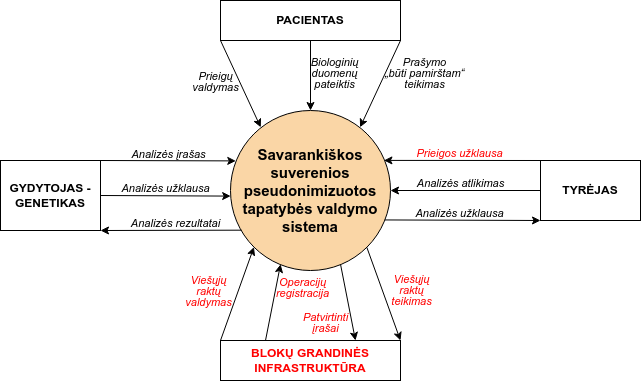
\includegraphics[width=1.0\linewidth]{Konteksto_diagrama.png}
        \vspace{-1\baselineskip}
        \caption{\small\textbf{Veiklos konteksto diagrama.}}
        \label{fig:context}
    \end{center}
\end{figure}

\subsection{Veiklos padalinimas}
Veiklos konteksto diagramos (\hyperref[fig:context]{1 pav.}) srautų
apibūdinimas:

\begin{enumerate}[itemsep=0.5pt]
    \item[\textbf{SR1:}] Pacientas įkelia savo biologinius duomenis.
    \item[\textbf{SR2:}] Gydytojas - genetikas sukuria analizės įrašą.
    \item[\textbf{SR3:}] Gydytojas - genetikas pateikia analizės užklausą
    tyrėjui.
    \item[\textbf{SR4:}] Tyrėjas gauna analizės užklausą iš gydytojo - genetiko.
    \item[\textbf{SR5:}] Esant poreikiui, tyrėjas pateikia prieigos užklausą
    pacientui, kad galėtų dirbti su paciento biologiniais duomenimis.
    \item[\textbf{SR6:}] Pacientas suteikia arba atmeta prieigos užklausą.
    \item[\textbf{SR7:}] Tyrėjas atlieka biologinių duomenų analizę.
    \item[\textbf{SR8:}] Tyrėjas pateikia analizės rezultatus, kuriuos gauna
    gydytojas - genetikas.
\end{enumerate}

\newpage

\section{Produkto veiklos sfera}
\subsection{Sistemos ribos}
Žemiau esančiame paveiksle pavaizduota sistemos panaudojimo atvejų diagrama:

\begin{figure}[ht]
    \begin{center}
        \captionsetup{justification=centering}
        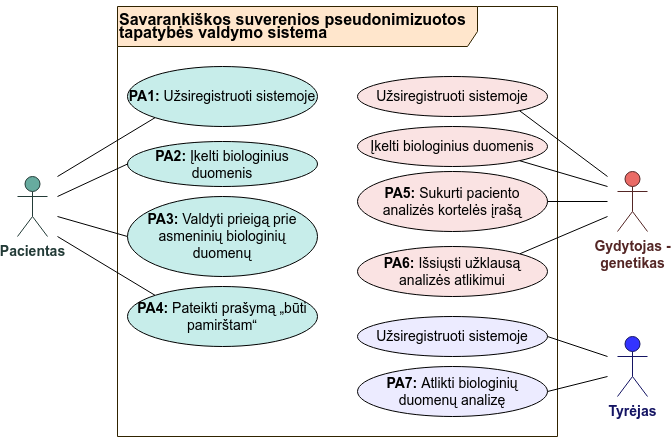
\includegraphics[width=0.9\linewidth]{PAM.png}
        \vspace{-1\baselineskip}
        \caption{\small\textbf{Panaudojimo atvejų modelis (PAM).}}
        \label{fig:image2}
    \end{center}
\end{figure}

\newpage

\subsection{Panaudojimo atvejų aprašymai}
Šiame skyriuje yra aprašyti visi kuriamos savarankiškos suverenios
pseudonimizuotos tapatybės valdymo sistemos panaudojimo atvejai.

\newpage

\hypertarget{PA1}{\noindent \textbf{PA1:} Užsiregistruoti sistemoje skirtingų
kategorijų naudotojams.}
\label{sec:PA1}
\begin{table}[htb!]
    \captionsetup{justification=centering}
    \begin{tabular}{|m{2.9cm}|m{14.3cm}|}
        \hline
        \raggedleft \textbf{\cellcolor{deepchampagne}Tikslas/ uždavinys} &
        Valdyti asmeninius duomenimis ir naudotis sistemoje realizuotu
        funkcionalumu, priklausomai nuo naudotojo kategorijos. \\
        \hline
        \raggedleft \textbf{\cellcolor{deepchampagne}Aprašymas} &
        Realizavus šį panaudojimo atvejį skirtingos naudotojų grupės sistemoje
        gali atlikti skirtingus veiksmus: pacientai gali įkelti savo biologinius
        duomenis ir valdyti kitų asmenų prieigą prie šių duomenų; gydytojai -
        genetikai gali kurti pacientų analizių korteles, bet ir įkelti pacientų
        biologinius duomenis, teikti užklausas tyrėjams dėl biologinių duomenų
        analizės atlikimo, peržiūrėti analizių atlikimo statusą; tyrėjai gali
        vykdyti biologinių duomenų analizes ir teikti jų rezultatus gydytojams -
        genetikams. \\
        \hline
        \raggedleft \textbf{\cellcolor{deepchampagne}Prioritetas} & Aukštas. \\
        \hline
        \raggedleft \textbf{\cellcolor{deepchampagne}Užsakovo (ne)tenkinimas} &
        Netenkinimas: 5, tenkinimas: 5. \\
        \hline
        \raggedleft \textbf{\cellcolor{deepchampagne}Aktorius} &
        Pacientas, gydytojas - genetikas, tyrėjas. \\
        \hline
        \raggedleft \textbf{\cellcolor{deepchampagne}Prieš - sąlyga} &
        Sistemos naudotojas turi būti atsidaręs pradinį sistemos langą. \\
        \hline
        \raggedleft \textbf{\cellcolor{deepchampagne}Sužadinimo sąlyga} &
        Sistemos naudotojas atsidaro sistemos langą, kuriame pateikta
        asmeninės paskyros kūrimo - registracijos - forma. \\
        \hline
        \raggedleft \textbf{\cellcolor{deepchampagne}Pagrindinis
        scenarijus\footnote{Čia ir toliau \textcolor{dartmouthgreen}{žalia}
        spalva pažymėti naudotojo veiksmai.}} & \vskip 5pt
        \makecell[l]{\parbox[t]{13.7cm}{
            \textbf{1.} \textcolor{dartmouthgreen}{Užpildomi pateiktos
            asmeninės paskyros kūrimo formos laukai.} \\
            \textbf{2.} \textcolor{dartmouthgreen}{Išsaugoma įvesta
            informacija, paspaudžiant išsaugojimo mygtuką.} \\
            \textbf{3.} Sistema patikrina, ar užpildyti visi privalomi asmeninės
            paskyros kūrimo formos laukai.
            \\
            \textbf{4.} {Jei visi privalomi asmeninės paskyros kūrimo formos
            laukai yra užpildyti, tuomet:} \\
            \textbf{5.} {Duomenų bazėje sukuriamas naujas sistemos naudotojas, o
            jo asmeniniai duomenys yra užšifruojami jiems priskiriant
            pseudonimus.} \\
            \textbf{6.} {Parodomas informacinis
            pranešimas, informuojantis apie sėkmingai sukurtą asmeninę
            paskyrą.} \\
            \textbf{7.} {Naudotojui atidaromas jo asmeninės paskyros langas.} \\
            \textbf{8. Baigiamas PA.}
        }}
        \\
        \hline
        \raggedleft \textbf{\cellcolor{deepchampagne}Po - sąlyga} &
        Duomenų bazėje sukuriamas naujas sistemos naudotojas, galintis
        prisijungti prie sistemos ir, pagal naudotojo kategoriją, naudotis
        sistemos funkcionalumu. \\
        \hline
        \raggedleft \textbf{\cellcolor{deepchampagne}Alternatyvūs scenarijai} &
        \vskip 5pt
        \makecell[l]{\parbox[t]{13.7cm}{
            \textbf{1.} \textcolor{dartmouthgreen}{Užpildomi pateiktos
            asmeninės paskyros kūrimo formos laukai.} \\
            \textbf{2.} \textcolor{dartmouthgreen}{Išsaugoma įvesta
            informacija, paspaudžiant išsaugojimo mygtuką.} \\
            \textbf{3.} Parodomas informacinis pranešimas, informuojantis, kad
            neužpildyti visi privalomi asmeninės paskyros kūrimo formos
            laukai. \\
            \textbf{4.} \textcolor{dartmouthgreen}{Užpildomi trūkstami
            asmeninės paskyros kūrimo formos laukai.} \\
            \textbf{5.} \textcolor{dartmouthgreen}{Išsaugoma įvesta
            informacija, paspaudžiant išsaugojimo mygtuką.} \\
            \textbf{6.} {Naudotojui atidaromas jo asmeninės paskyros langas.} \\
            \textbf{7. Baigiamas PA.}
        }}
        \\
        \hline
    \end{tabular}
\end{table}

\newpage

\hypertarget{PA2}\noindent \textbf{PA2:} Įkelti biologinius duomenis.
\label{sec:PA2}
\begin{table}[htb!]
    \captionsetup{justification=centering}
    \begin{tabular}{|m{3cm}|m{13.7cm}|}
        \hline
        \raggedleft \textbf{\cellcolor{deepchampagne}Tikslas/ uždavinys} &
        Pateikti biologinius duomenis, kurie gali būti panaudoti, siekiant
        išsiaiškinti ligų priežastis, arba moksliniais tikslais. \\
        \hline
        \raggedleft \textbf{\cellcolor{deepchampagne}Aprašymas} &
        Realizavus šį panaudojimo atvejį skirtingos naudotojų grupės sistemoje
        gali atlikti tą patį veiksmą, turint skirtingų siekių: pacientai gali
        įkelti savo biologinius duomenis, kurie gali būti panaudoti moksliniais
        tikslais, papildant biologinių duomenų saugyklą naujais genetiniais
        variantais; gydytojai - genetikai gali įkelti genetinius pacientų
        duomenis, kad jie būtų detaliau išanalizuoti tyrėjų ir būtų galima
        paskirti tolimesnes sutrikimo ar ligos gydymo priemones. \\
        \hline
        \raggedleft \textbf{\cellcolor{deepchampagne}Prioritetas} & Aukštas. \\
        \hline
        \raggedleft \textbf{\cellcolor{deepchampagne}Užsakovo (ne)tenkinimas} &
        Netenkinimas: 5, tenkinimas: 5. \\
        \hline
        \raggedleft \textbf{\cellcolor{deepchampagne}Aktorius} &
        Pacientas, gydytojas - genetikas. \\
        \hline
        \raggedleft \textbf{\cellcolor{deepchampagne}Prieš - sąlyga} &
        Sistemos naudotojas turi būti prisijungęs prie sistemos. \\
        \hline
        \raggedleft \textbf{\cellcolor{deepchampagne}Sužadinimo sąlyga} &
        Sistemos naudotojas atsidaro sistemos langą, kuriame pateikta
        biologinių duomenų įkėlimo skiltis su metaduomenų įvedimo forma. \\
        \hline
        \raggedleft \textbf{\cellcolor{deepchampagne}Pagrindinis
        scenarijus} & \vskip 5pt
        \makecell[l]{\parbox[t]{13.7cm}{
            \textbf{1.} \textcolor{dartmouthgreen}{Užpildomi pateiktos duomenų
            įkėlimo formos laukai ir pridedamas biologinius duomenis saugantis
            failas.} \\
            \textbf{2.} \textcolor{dartmouthgreen}{Išsaugoma įvesta
            metainformacija bei pridėtas failas, paspaudžiant išsaugojimo
            mygtuką.} \\
            \textbf{3.} {Validuojamas failo formatas ir turinys.} \\
            \textbf{4.} {Duomenys užšifruojami ir išsaugomi duomenų bazėje.} \\
            \textbf{5.} {Metainformacija apie įkeltą failą įrašoma į blokų
            grandinę (taip užtikrinant duomenų nekintamumą ir veiksmų
            atsekamumą).} \\
            \textbf{6.} {Biologinių duomenų įrašui priskiriamas unikalus
            identifikatorius ir susiejamas su naudotojo paskyra.} \\
            \textbf{7.} {Parodomas informacinis pranešimas, informuojantis apie
            sėkmingai įkeltus duomenis.} \\
            \textbf{8.} \textcolor{dartmouthgreen}{Atveriama naudotojo paskyros
            skiltis su įkeltų duomenų įrašu.} \\
            \textbf{9. Baigiamas PA.}
        }}
        \\
        \hline
        \raggedleft \textbf{\cellcolor{deepchampagne}Po - sąlyga} &
        Į duomenų bazę įkeliami užšifruoti biologiniai duomenys. \\
        \hline
        \raggedleft \textbf{\cellcolor{deepchampagne}Alternatyvūs scenarijai} &
        \vskip 5pt
        \makecell[l]{\parbox[t]{13.7cm}{
            \textbf{1.} \textcolor{dartmouthgreen}{Užpildomi pateiktos
            duomenų įkėlimo formos laukai ir pridedamas biologinius duomenis
            saugantis failas.} \\
            \textbf{2.} \textcolor{dartmouthgreen}{Išsaugoma įvesta
            metainformacija bei pridėtas failas, paspaudžiant išsaugojimo
            mygtuką.} \\
            \textbf{3.} {Validuojamas failo formatas ir turinys.} \\
            \textbf{4.} {Įkeltas failas dėl vidinės klaidos nesėkmingai
            užšifruojamas.} \\
            \textbf{5.} {Parodomas informacinis pranešimas, informuojantis, kad
            duomenų įkėlimas buvo nesėkmingas.} \\
            \textbf{6.} {Naudotojui pasiūloma pakartoti duomenų įkėlimo
            veiksmą.} \\
            \textbf{7. Baigiamas PA.}
        }}
        \\
        \hline
    \end{tabular}
\end{table}

\newpage

\noindent \textbf{PA3:} Valdyti prieigą prie asmeninių biologinių duomenų.
\label{sec:PA3}
\begin{table}[htb!]
    \captionsetup{justification=centering}
    \begin{tabular}{|m{3cm}|m{13.7cm}|}
        \hline
        \raggedleft \textbf{\cellcolor{deepchampagne}Tikslas/ uždavinys} &
        Suteikti galimybę naudotojui (pacientui) nuspręsti, ar jo pateikti
        asmeniniai biologiniai duomenys gali būti prieinami kitiems
        naudotojams (gydytojams - genetikams ir tyrėjams). Prieigą prie
        asmeninių biologinių duomenų valdantis asmuo gali suteikti prieigą arba
        atmesti užklausą dėl duomenų prieigos. \\
        \hline
        \raggedleft \textbf{\cellcolor{deepchampagne}Aprašymas} &
        Realizavus šį panaudojimo atvejį skirtingos naudotojų grupės
        (gydytojai - genetikai, tyrėjai) gali vykdyti analizes su pateiktais
        biologiniais duomenimis bei daryti išvadas apie paciento sveikatos
        būklę. Jeigu gydytojai - genetikai arba tyrėjai netenka prieigos
        prie pacientų biologinių duomenų, tolimesnė duomenų analizė yra
        negalima. \\
        \hline
        \raggedleft \textbf{\cellcolor{deepchampagne}Prioritetas} & Aukštas. \\
        \hline
        \raggedleft \textbf{\cellcolor{deepchampagne}Užsakovo (ne)tenkinimas} &
        Netenkinimas: 5, tenkinimas: 5. \\
        \hline
        \raggedleft \textbf{\cellcolor{deepchampagne}Aktorius} &
        Pacientas. \\
        \hline
        \raggedleft \textbf{\cellcolor{deepchampagne}Prieš - sąlyga} &
        Sistemos naudotojas turi būti prisijungęs prie sistemos. \\
        \hline
        \raggedleft \textbf{\cellcolor{deepchampagne}Sužadinimo sąlyga} &
        Sistemos naudotojas atsidaro sistemos langą, kuriame realizuotas duomenų
        prieigos valdymo funkcionalumas. \\
        \hline
        \raggedleft \textbf{\cellcolor{deepchampagne}Pagrindinis
        scenarijus} & \vskip 5pt
        \makecell[l]{\parbox[t]{13.7cm}{
            \textbf{1.} {Sistema pateikia paciento
            įkeltų biologinių duomenų sąrašą.} \\
            \textbf{2.} \textcolor{dartmouthgreen}{Pasirenkamas konkretus
            biologinių duomenų sąrašo įrašas.} \\
            \textbf{3.} {Pateikiamas naudotojų, turinčių prieigą prie konkrečių
            biologinių duomenų, sąrašas.} \\
            \textbf{4.} \textcolor{dartmouthgreen}{Redaguojamos sistemos
            naudotojams suteiktos prieigos teisės: pratęsiamas prieigos
            laikotarpis arba atšaukiama prieiga.} \\
            \textbf{5.} \textcolor{dartmouthgreen}{Suteikiamos naujos prieigos
            naujiems sistemos naudotojams.} \\
            \textbf{6.} {Atnaujinamas naudotojams suteiktų prieigų sąrašas.} \\
            \textbf{7.} {Įrašo pakeitimo informacija išsaugoma į blokų
            grandinę.} \\
            \textbf{8.} {Parodomas informacinis pranešimas, informuojantis apie
            sėkmingai atliktą atnaujinimą.} \\
            \textbf{9.} {Sistema informuoja atitinkamus sistemos naudotojus apie
            prieigos teisių pasikeitimus.} \\
            \textbf{10. Baigiamas PA.}
        }}
        \\
        \hline
        \raggedleft \textbf{\cellcolor{deepchampagne}Po - sąlyga} &
        Sistemos naudotojams (gydytojams - genetikams, tyrėjams) yra suteikiama
        arba apribojama prieiga prie paciento biologinių duomenų. \\
        \hline
        \raggedleft \textbf{\cellcolor{deepchampagne}Alternatyvūs scenarijai} &
        \vskip 5pt
        \makecell[l]{\parbox[t]{13.7cm}{
            \textbf{1.} {Pateikiamas paciento įkeltų biologinių duomenų
            sąrašas.} \\
            \textbf{2.} \textcolor{dartmouthgreen}{Pasirenkamas konkretus
            biologinių duomenų sąrašo įrašas.} \\
            \textbf{3.} {Pateikiamas naudotojų, turinčių prieigą prie konkrečių
            biologinių duomenų, sąrašas.} \\
            \textbf{4.} \textcolor{dartmouthgreen}{Bandoma redaguoti suteiktas
            prieigos teises konkrečiam naudotojui.} \\
            \textbf{5.} \textcolor{dartmouthgreen}{Parodomas informacinis
            pranešimas, informuojantis apie nesėkmingą prieigos teisių
            atnaujinimą (tuo atveju, jei naudotojas neaktyvus - nebedirba
            įstaigoje, dirbančioje su kuriama sistema).} \\
            \textbf{6. Baigiamas PA.}
        }}
        \\
        \hline
    \end{tabular}
\end{table}

\newpage

\hypertarget{PA4}\noindent \textbf{PA4:} Pateikti prašymą „būti pamirštam“.
\label{sec:PA4}
\begin{table}[htb!]
    \captionsetup{justification=centering}
    \begin{tabular}{|m{3cm}|m{13.7cm}|}
        \hline
        \raggedleft \textbf{\cellcolor{deepchampagne}Tikslas/ uždavinys} &
        Leisti naudotojui (pacientui) pateikti prašymą dėl asmeninių ir įkeltų
        biologinių duomenų bei visų su jais susijusių įrašų panaikinimo iš
        saugyklų. \\
        \hline
        \raggedleft \textbf{\cellcolor{deepchampagne}Aprašymas} &
        Remiantis 17 BDAR straipsniu naudotojas turi galėti pateikti prašymą
        ištrinti visus jo pateiktus duomenis. Realizavus šį panaudojimo atvejį
        naudotojui iniciavus duomenų panaikinimą iš duomenų bazių yra ištrinami
        visi saugomi su pacientu susiję biologiniai duomenys bei su jais susiję
        įrašai. \\
        \hline
        \raggedleft \textbf{\cellcolor{deepchampagne}Prioritetas} & Aukštas. \\
        \hline
        \raggedleft \textbf{\cellcolor{deepchampagne}Užsakovo (ne)tenkinimas} &
        Netenkinimas: 3, tenkinimas: 5. \\
        \hline
        \raggedleft \textbf{\cellcolor{deepchampagne}Aktorius} &
        Pacientas. \\
        \hline
        \raggedleft \textbf{\cellcolor{deepchampagne}Prieš - sąlyga} &
        Sistemos naudotojas turi būti prisijungęs prie sistemos. \\
        \hline
        \raggedleft \textbf{\cellcolor{deepchampagne}Sužadinimo sąlyga} &
        Sistemos naudotojas atsidaro asmeninės paskyros peržiūros ir redagavimo
        sistemos langą. \\
        \hline
        \raggedleft \textbf{\cellcolor{deepchampagne}Pagrindinis
        scenarijus} & \vskip 5pt
        \makecell[l]{\parbox[t]{13.7cm}{
            \textbf{1.} \textcolor{dartmouthgreen}{Asmeninės paskyros redagavimo
            lange pažymima parinktis „Prašymas būti pamirštam“.} \\
            \textbf{2.} {Sistema pateikia pasekmių, susijusių su prašymo būti
            pamirštam išsiuntimu, sąrašą ir nurodo, kad reikalingas naudotojo
            patvirtinimas.} \\
            \textbf{3.} \textcolor{dartmouthgreen}{Naudotojas patvirtina, kad
            susipažino su pasekmėmis ir patvirtina prašymą.} \\
            \textbf{4.} {Sistema patikrina, ar einamuoju metu nėra atliekama
            paciento pateiktų biologinių duomenų analizė.} \\
            \textbf{5.} {Sistema panaikina naudotojo asmeninius duomenis, visų
            naudotojų prieigas prie biologinių duomenų, ištrina visus su
            naudotoju susijusius duomenis iš duomenų bazių ir užfiksuoja
            „pamiršimo“ įvykį blokų grandinėje.} \\
            \textbf{6.} {Parodomas informacinis pranešimas, informuojantis apie
            sėkmingai įgyvendintą prašymą būti pamirštam.} \\
            \textbf{7. Baigiamas PA.}
        }}
        \\
        \hline
        \raggedleft \textbf{\cellcolor{deepchampagne}Po - sąlyga} &
        Naudotojo duomenys yra pašalinti, biologiniai duomenys yra nebeprieinami
        kitiems sistemos naudotojams. \\
        \hline
        \raggedleft \textbf{\cellcolor{deepchampagne}Alternatyvūs scenarijai} &
        \vskip 5pt
        \makecell[l]{\parbox[t]{13.7cm}{
            \textbf{1.} \textcolor{dartmouthgreen}{Asmeninės paskyros redagavimo
            lange pažymima parinktis „Prašymas būti pamirštam“.} \\
            \textbf{2.} {Sistema pateikia pasekmių,
            susijusių su prašymo būti pamirštam išsiuntimu, sąrašą ir
            nurodo, kad reikalingas naudotojo patvirtinimas.} \\
            \textbf{3.} \textcolor{dartmouthgreen}{Naudotojas patvirtina, kad
            susipažino su pasekmėmis ir patvirtina prašymą.} \\
            \textbf{4.} {Sistema patikrina, ar
            einamuoju metu nėra atliekama paciento pateiktų biologinių duomenų
            analizė.} \\
            \textbf{5.} {Sistema nustato, kad su
            biologiniais duomenimis tebėra atliekami tyrimai.} \\
            \textbf{6.} {Parodomas informacinis
            pranešimas, informuojantis apie einamuoju metu negalimą prašymo
            būti pamirštam įgyvendinimą.} \\
            \textbf{7. Baigiamas PA.}
        }}
        \\
        \hline
    \end{tabular}
\end{table}

\newpage

\hypertarget{PA5}\noindent \textbf{PA5:} Sukurti paciento analizės kortelės
įrašą.
\label{sec:PA5}
\begin{table}[htb!]
    \captionsetup{justification=centering}
    \begin{tabular}{|m{3cm}|m{13.7cm}|}
        \hline
        \raggedleft \textbf{\cellcolor{deepchampagne}Tikslas/ uždavinys} &
        Leisti gydytojui - genetikui sukurti naują paciento kortelės įrašą su
        informacija apie analize.\\
        \hline
        \raggedleft \textbf{\cellcolor{deepchampagne}Aprašymas} &
        Realizavus šį panaudojimo atvejį yra sukuriamas paciento medicininės
        kortelės įrašas, kuriame, esant poreikiui, užfiksuojami paciento
        biologiniai duomenys, pateikiami preliminarūs klinikiniai duomenys,
        aprašoma reikalinga analizė ir įrašomi analizės rezultatai. \\
        \hline
        \raggedleft \textbf{\cellcolor{deepchampagne}Prioritetas} & Aukštas. \\
        \hline
        \raggedleft \textbf{\cellcolor{deepchampagne}Užsakovo (ne)tenkinimas} &
        Netenkinimas: 5, tenkinimas: 5. \\
        \hline
        \raggedleft \textbf{\cellcolor{deepchampagne}Aktorius} &
        Gydytojas - genetikas. \\
        \hline
        \raggedleft \textbf{\cellcolor{deepchampagne}Prieš - sąlyga} &
        Sistemos naudotojas turi būti prisijungęs prie sistemos. \\
        \hline
        \raggedleft \textbf{\cellcolor{deepchampagne}Sužadinimo sąlyga} &
        Sistemos naudotojas atsidaro paciento kortelės įrašų kūrimo langą. \\
        \hline
        \raggedleft \textbf{\cellcolor{deepchampagne}Pagrindinis
        scenarijus} & \vskip 5pt
        \makecell[l]{\parbox[t]{13.7cm}{
            \textbf{1.} \textcolor{dartmouthgreen}{Naudotojas užpildo kortelės
            įrašo formos laukus.} \\
            \textbf{2.} \textcolor{dartmouthgreen}{Naudotojas išsaugo įvestus
            duomenis, paspausdamas išsaugojimo mygtuką.} \\
            \textbf{3.} Parodomas informacinis pranešimas, informuojantis apie
            sėkmingai sukurtą paciento kortelės įrašą. \\
            \textbf{4. Baigiamas PA.}
        }}
        \\
        \hline
        \raggedleft \textbf{\cellcolor{deepchampagne}Po - sąlyga} &
        Analizės užklausa yra užregistruota ir sėkmingai perduota tyrėjo
        vykdymui. \\
        \hline
        \raggedleft \textbf{\cellcolor{deepchampagne}Alternatyvūs scenarijai} &
        \vskip 5pt
        \makecell[l]{\parbox[t]{13.7cm}{
            \textbf{1.} \textcolor{dartmouthgreen}{Naudotojas užpildo kortelės
            įrašo formos laukus.} \\
            \textbf{2.} \textcolor{dartmouthgreen}{Naudotojas išsaugo įvestus
            duomenis, paspausdamas išsaugojimo mygtuką.} \\
            \textbf{3.} Parodomas informacinis pranešimas, informuojantis, kad
            neužpildyti visi privalomi kortelės įrašo kūrimo formos laukai. \\
            \textbf{4. Baigiamas PA.}
        }}
        \\
        \hline
    \end{tabular}
\end{table}

\newpage

\hypertarget{PA6}\noindent \textbf{PA6:} Išsiųsti užklausą analizės atlikimui.
\label{sec:PA6}
\begin{table}[htb!]
    \captionsetup{justification=centering}
    \begin{tabular}{|m{3cm}|m{13.7cm}|}
        \hline
        \raggedleft \textbf{\cellcolor{deepchampagne}Tikslas/ uždavinys} &
        Leisti gydytojui - genetikui pateikti prašymą tyrėjui atlikti paciento
        biologinių duomenų analizę. \\
        \hline
        \raggedleft \textbf{\cellcolor{deepchampagne}Aprašymas} &
        Realizavus šį panaudojimo atvejį yra išsiunčiamas prašymas biologinių
        duomenų savininkui, kad patvirtintų, ar jis sutinka, kad jo
        biologiniai duomenys būtų analizuojami tyrėjo. Gavus paciento leidimą
        yra informuojamas tyrėjas, kad reikalingas biologinių duomenų analizės
        atlikimas. \\
        \hline
        \raggedleft \textbf{\cellcolor{deepchampagne}Prioritetas} & Aukštas. \\
        \hline
        \raggedleft \textbf{\cellcolor{deepchampagne}Užsakovo (ne)tenkinimas} &
        Netenkinimas: 5, tenkinimas: 5. \\
        \hline
        \raggedleft \textbf{\cellcolor{deepchampagne}Aktorius} &
        Gydytojas - genetikas. \\
        \hline
        \raggedleft \textbf{\cellcolor{deepchampagne}Prieš - sąlyga} &
        Sistemos naudotojas turi būti prisijungęs prie sistemos. \\
        \hline
        \raggedleft \textbf{\cellcolor{deepchampagne}Sužadinimo sąlyga} &
        Sistemos naudotojas atsidaro paciento kortelės įrašų kūrimo langą. \\
        \hline
        \raggedleft \textbf{\cellcolor{deepchampagne}Pagrindinis
        scenarijus} & \vskip 5pt
        \makecell[l]{\parbox[t]{13.7cm}{
            \textbf{1.} \textcolor{dartmouthgreen}{Naudotojas pasirenka analizės
            pateikimo užklausos funkciją.} \\
            \textbf{2.} {Sistema pateikia paciento
            biologinių duomenų, kuriuos galima analizuoti sąrašą.} \\
            \textbf{3.} \textcolor{dartmouthgreen}{Naudotojas pasirenka
            aktualius biologinius duomenis bei įveda kitą su analize susijusią
            informaciją.} \\
            \textbf{4.} {Sistema pateikia tyrėjų, kurie
            gali atlikti analizę, sąrašą.} \\
            \textbf{5.} \textcolor{dartmouthgreen}{Naudotojas pasirenka tyrėją ir
            išsiunčia užklausą pasirinktam tyrėjui.} \\
            \textbf{6.} {Sistema patikrina, ar gydytojas
            ir pasirinktas tyrėjas turi prieigą prie paciento duomenų.} \\
            \textbf{7.} {Sistema užšifruoja užklausą,
            išsaugo ją duomenų bazėje ir išsiunčia parinktam tyrėjui.} \\
            \textbf{8.} {Parodomas informacinis
            pranešimas, informuojantis apie sėkmingai išsiųstą užklausą.} \\
            \textbf{9.} \textcolor{dartmouthgreen}{Naudotojas gali stebėti
            analizės atlikimo būseną.} \\
            \textbf{10. Baigiamas PA.}
        }}
        \\
        \hline
        \raggedleft \textbf{\cellcolor{deepchampagne}Po - sąlyga} &
        Analizės užklausa yra užregistruota ir sėkmingai perduota tyrėjo
        vykdymui. \\
        \hline
        \raggedleft \textbf{\cellcolor{deepchampagne}Alternatyvūs scenarijai} &
        \vskip 5pt
        \makecell[l]{\parbox[t]{13.7cm}{
            \textbf{1.} \textcolor{dartmouthgreen}{Naudotojas pasirenka analizės
            pateikimo užklausos funkciją.} \\
            \textbf{2.} {Sistema pateikia paciento
            biologinių duomenų, kuriuos galima analizuoti sąrašą.} \\
            \textbf{3.} \textcolor{dartmouthgreen}{Naudotojas pasirenka
            aktualius biologinius duomenis bei įveda kitą su analize susijusią
            informaciją.} \\
            \textbf{4.} {Sistema pateikia tyrėjų, kurie
            gali atlikti analizę, sąrašą.} \\
            \textbf{5.} \textcolor{dartmouthgreen}{Naudotojas pasirenka tyrėją
            ir išsiunčia užklausą pasirinktam tyrėjui.} \\
            \textbf{6.} {Sistema patikrina, ar gydytojas
            ir pasirinktas tyrėjas turi prieigą prie paciento duomenų.} \\
            \textbf{7.} {Parodomas informacinis
            pranešimas, informuojantis apie negalimą užklausos išsiuntimą dėl
            duomenų prieigos teisių neturėjimo.} \\
            \textbf{8. Baigiamas PA.}
        }}
        \\
        \hline
    \end{tabular}
\end{table}

\newpage

\hypertarget{PA7}\noindent \textbf{PA7:} Atlikti biologinių duomenų analizę.
\label{sec:PA7}
\begin{table}[htb!]
    \captionsetup{justification=centering}
    \begin{tabular}{|m{3cm}|m{13.7cm}|}
        \hline
        \raggedleft \textbf{\cellcolor{deepchampagne}Tikslas/ uždavinys} &
        Išanalizuoti paciento biologinius duomenis bei pateikti įžvalgas apie
        juos. \\
        \hline
        \raggedleft \textbf{\cellcolor{deepchampagne}Aprašymas} &
        Realizavus šį panaudojimo atvejį yra įgyvendinama gydytojo - genetiko
        tyrėjui pateikta užklausa dėl biologinių duomenų analizės atlikimo. \\
        \hline
        \raggedleft \textbf{\cellcolor{deepchampagne}Prioritetas} & Aukštas. \\
        \hline
        \raggedleft \textbf{\cellcolor{deepchampagne}Užsakovo (ne)tenkinimas} &
        Netenkinimas: 5, tenkinimas: 5. \\
        \hline
        \raggedleft \textbf{\cellcolor{deepchampagne}Aktorius} &
        Tyrėjas. \\
        \hline
        \raggedleft \textbf{\cellcolor{deepchampagne}Prieš - sąlyga} &
        Sistemos naudotojas turi būti prisijungęs prie sistemos. \\
        \hline
        \raggedleft \textbf{\cellcolor{deepchampagne}Sužadinimo sąlyga} &
        Sistemos naudotojas atsidaro gautą analizės atlikimo užklausą. \\
        \hline
        \raggedleft \textbf{\cellcolor{deepchampagne}Pagrindinis
        scenarijus} & \vskip 5pt
        \makecell[l]{\parbox[t]{13.7cm}{
            \textbf{1.} \textcolor{dartmouthgreen}{Naudotojas peržiūri gautus
            pseudonimizuotus ir užšifruotus biologinius duomenis.} \\
            \textbf{2.} \textcolor{dartmouthgreen}{Naudotojas pasirenka tinkamą
            analizės metodą, naudodamasis integruota arba išorine analizės
            vykdymo programine įranga.} \\
            \textbf{3.} \textcolor{dartmouthgreen}{Naudotojas įkelia analizės
            rezultatus į sistemą.} \\
            \textbf{4.} Sistema informuoja gydytoją - genetiką apie gautus
            analizės rezultatus. \\
            \textbf{5.} Sistema įrašo analizės rezultatą konkretaus paciento
            medicininės kortelės įraše. \\
            \textbf{6. Baigiamas PA.}
        }}
        \\
        \hline
        \raggedleft \textbf{\cellcolor{deepchampagne}Po - sąlyga} &
        Analizės užklausa yra užregistruota ir sėkmingai perduota tyrėjo
        vykdymui. \\
        \hline
        \raggedleft \textbf{\cellcolor{deepchampagne}Alternatyvūs scenarijai} &
        \vskip 5pt
        \makecell[l]{\parbox[t]{13.7cm}{
            \textbf{1.} \textcolor{dartmouthgreen}{Naudotojas peržiūri gautus
            pseudonimizuotus ir užšifruotus biologinius duomenis.} \\
            \textbf{2.} \textcolor{dartmouthgreen}{Naudotojas pasirenka tinkamą
            analizės metodą, naudodamasis integruota arba išorine analizės
            vykdymo programine įranga.} \\
            \textbf{3.} \textcolor{dartmouthgreen}{Atliekant analizę paaiškėja,
            kad pateikti biologiniai duomenys yra nepakankami arba netinkami,
            todėl gydytojo - genetiko siųsta analizės atlikimo užklausa yra
            atmetama, pateikiant detalias atmetimo priežastis.} \\
            \textbf{4. Baigiamas PA.}
        }}
        \\
        \hline
    \end{tabular}
\end{table}

\newpage

\section{Funkciniai reikalavimai ir reikalavimai duomenims}
\subsection{Funkciniai reikalavimai}
Šiame skyriuje yra aprašyti visi kuriamos sistemos funkciniai reikalavimai bei
su jais susieti panaudojimo atvejai.

\vskip 10pt

\hypertarget{FR1}\noindent \textbf{FR1:} Registracijos formos pateikimas.
\label{sec:FR1}
\begin{table}[htb!]
    \captionsetup{justification=centering}
    \begin{tabular}{|m{4.8cm}|m{12cm}|}
        \hline
        \raggedleft \textbf{\cellcolor{deepchampagne}Aprašymas} & Sistema turi
        pateikti registracijos formą, kurioje naudotojas turi galėti įvesti
        privalomus duomenis: vardą, pavardę, el. pašto adresą arba telefono
        numerį bei pasirinkti savo naudotojo kategoriją. \\
        \hline
        \raggedleft \textbf{\cellcolor{deepchampagne}Pagrindimas} & Tam, jog
        būtų sukurta naudotojo paskyra, turi būti įvesta ir išsaugota
        informacija apie naudotoją. \\
        \hline
        \raggedleft \textbf{\cellcolor{deepchampagne}Šaltinis} & Užsakovas. \\
        \hline
        \raggedleft \textbf{\cellcolor{deepchampagne}Tikimo kriterijus} &
        Sistemos registracijos formos lauke atvaizduojama registracijos forma
        su išskirtais privalomais įvesties laukais. \\
        \hline
        \raggedleft \textbf{\cellcolor{deepchampagne}Užsakovo (ne)tenkinimas} &
        Netenkinimas: 5, tenkinimas: 5. \\
        \hline
        \raggedleft \textbf{\cellcolor{deepchampagne}Priklausomybės} &
        \begin{itemize}[leftmargin=0.3cm, itemsep=-7pt, topsep=1pt,
                            after=\vspace{-1em}]
            \item \hyperlink{FR2}{\textcolor{steelblue}{\textbf{FR2:} Naudotojo
            kategorijos pasirinkimas}}
            \item \hyperlink{FR3}{\textcolor{steelblue}{\textbf{FR3:} Formų
            validavimas}}
        \end{itemize}
        \\
        \hline
        \raggedleft \textbf{\cellcolor{deepchampagne}Susijęs panaudojimo
        atvejis} &
        \hyperlink{PA1}{\textcolor{steelblue}{\textbf{PA1:} Užsiregistruoti
        sistemoje skirtingų kategorijų naudotojams}} \\
        \hline
    \end{tabular}
\end{table}

\hypertarget{FR2}\noindent \textbf{FR2:} Naudotojo kategorijos pasirinkimas.
\label{sec:FR2}
\begin{table}[htb!]
    \captionsetup{justification=centering}
    \begin{tabular}{|m{4.8cm}|m{12cm}|}
        \hline
        \raggedleft \textbf{\cellcolor{deepchampagne}Aprašymas} & Sistema
        turi leisti registracijos formoje pasirinkti naudotojo kategoriją
        iš 3 galimų: „gydytojas - genetikas“, „tyrėjas“, „pacientas“. \\
        \hline
        \raggedleft \textbf{\cellcolor{deepchampagne}Pagrindimas} & Priklausomai
        nuo to, kokia yra naudotojo kategorija, naudotojui yra prieinamas
        skirtingas sistemos funkcionalumas. \\
        \hline
        \raggedleft \textbf{\cellcolor{deepchampagne}Šaltinis} & Užsakovas. \\
        \hline
        \raggedleft \textbf{\cellcolor{deepchampagne}Tikimo kriterijus} &
        Registracijos formoje leidžiama pasirinkti naudotojo kategoriją. \\
        \hline
        \raggedleft \textbf{\cellcolor{deepchampagne}Užsakovo (ne)tenkinimas} &
        Netenkinimas: 5, tenkinimas: 5. \\
        \hline
        \raggedleft \textbf{\cellcolor{deepchampagne}Priklausomybės} &
        \hyperlink{FR1}{\textcolor{steelblue}{\textbf{FR1:} Registracijos formos
        pateikimas}} \\
        \hline
        \raggedleft \textbf{\cellcolor{deepchampagne}Susijęs panaudojimo
        atvejis} &
        \hyperlink{PA1}{\textcolor{steelblue}{\textbf{PA1:} Užsiregistruoti
        sistemoje skirtingų kategorijų naudotojams}} \\
        \hline
    \end{tabular}
\end{table}

\newpage

\hypertarget{FR3}\noindent \textbf{FR3:} Formų validavimas.
\label{sec:FR3}
\begin{table}[htb!]
    \captionsetup{justification=centering}
    \begin{tabular}{|m{4.8cm}|m{12cm}|}
        \hline
        \raggedleft \textbf{\cellcolor{deepchampagne}Aprašymas} & Sistema
        turi validuoti privalomus formų laukus ir neleisti išsaugoti įvestos
        informacijos tol, kol nebus pateikta visa būtina teisinga
        informacija. \\
        \hline
        \raggedleft \textbf{\cellcolor{deepchampagne}Pagrindimas} & Formų
        validavimas padeda užtikrinti korektiškų duomenų saugojimą duomenų
        bazėje bei užtikrina, kad bus pateikta visa aktuali informacija apie
        sistemos naudotoją. \\
        \hline
        \raggedleft \textbf{\cellcolor{deepchampagne}Šaltinis} & Užsakovas. \\
        \hline
        \raggedleft \textbf{\cellcolor{deepchampagne}Tikimo kriterijus} &
        Formose nepateikus visos būtinos informacijos pateikiami aiškūs
        validaciniai pranešimai; įvesti duomenys neišsaugomi duomenų bazėje. \\
        \hline
        \raggedleft \textbf{\cellcolor{deepchampagne}Užsakovo (ne)tenkinimas} &
        Netenkinimas: 5, tenkinimas: 5. \\
        \hline
        \raggedleft \textbf{\cellcolor{deepchampagne}Priklausomybės} &
        \hyperlink{FR1}{\textcolor{steelblue}{\textbf{FR1:} Registracijos formos
        pateikimas}} \\
        \hline
        \raggedleft \textbf{\cellcolor{deepchampagne}Susijęs panaudojimo
        atvejis} &
        \hyperlink{PA1}{\textcolor{steelblue}{\textbf{PA1:} Užsiregistruoti
        sistemoje skirtingų kategorijų naudotojams}} \\
        \hline
    \end{tabular}
\end{table}

\hypertarget{FR4}\noindent \textbf{FR4:} Informacijos išsaugojimas.
\label{sec:FR4}
\begin{table}[htb!]
    \captionsetup{justification=centering}
    \begin{tabular}{|m{4.8cm}|m{12cm}|}
        \hline
        \raggedleft \textbf{\cellcolor{deepchampagne}Aprašymas} & Sistemoje
        įvedus duomenis, įkėlus biologinių duomenų failus, atlikus biologinę
        analizę arba pateikus užklausą dėl analizės atlikimo paspaudus
        duomenų išsaugojimo mygtuką visi duomenys turi būti išsaugoti
        atitinkamose duomenų bazės lentelėse. \\
        \hline
        \raggedleft \textbf{\cellcolor{deepchampagne}Pagrindimas} & Naudotojų
        pateikta informacija privalo būti išsaugota, kad ji galėtų būti
        tikslingai panaudota, atliekant skirtingas sistemos funkcijas. \\
        \hline
        \raggedleft \textbf{\cellcolor{deepchampagne}Šaltinis} & Užsakovas. \\
        \hline
        \raggedleft \textbf{\cellcolor{deepchampagne}Tikimo kriterijus} &
        Po išsaugojimo mygtuko paspaudimo visi naudotojų pateikti duomenys
        sėkmingai įrašomi ir atvaizduojami duomenų bazės lentelėse. \\
        \hline
        \raggedleft \textbf{\cellcolor{deepchampagne}Užsakovo (ne)tenkinimas} &
        Netenkinimas: 5, tenkinimas: 5. \\
        \hline
        \raggedleft \textbf{\cellcolor{deepchampagne}Priklausomybės} &
        \begin{itemize}[leftmargin=0.3cm, itemsep=-7pt, topsep=1pt,
                            after=\vspace{-1em}]
            \item \hyperlink{FR5}{\textcolor{steelblue}{\textbf{FR5:}
            Informavimas apie sėkmingai atliktą veiksmą}}
            \item \hyperlink{FR6}{\textcolor{steelblue}{\textbf{FR6:}
            Informavimas apie nesėkmingai atliktą veiksmą}}
        \end{itemize}
        \\
        \hline
        \raggedleft \textbf{\cellcolor{deepchampagne}Susijęs panaudojimo
        atvejis} &
        \begin{itemize}[leftmargin=0.3cm, itemsep=-7pt, topsep=1pt,
                            after=\vspace{-1em}]
            \item \hyperlink{PA1}{\textcolor{steelblue}{\textbf{PA1:}
            Užsiregistruoti sistemoje skirtingų kategorijų naudotojams}} 
        \end{itemize}
        \\
        \hline
    \end{tabular}
\end{table}

\newpage

\hypertarget{FR5}\noindent \textbf{FR5:} Informavimas apie sėkmingai atliktą
veiksmą.
\label{sec:FR5}
\begin{table}[htb!]
    \captionsetup{justification=centering}
    \begin{tabular}{|m{4.8cm}|m{12cm}|}
        \hline
        \raggedleft \textbf{\cellcolor{deepchampagne}Aprašymas} & Sistemoje
        turi būti parodomas pranešimas, informuojantis apie sėkmingai
        atliktą įrašymo į duomenų bazę (išsaugojimo) veiksmą. \\
        \hline
        \raggedleft \textbf{\cellcolor{deepchampagne}Pagrindimas} & Naudotojas
        turi žinoti, ar pateikus reikalingus duomenis ir iniciavus duomenų
        išsaugojimą šis veiksmas buvo sėkmingai įvykdytas. \\
        \hline
        \raggedleft \textbf{\cellcolor{deepchampagne}Šaltinis} & Užsakovas. \\
        \hline
        \raggedleft \textbf{\cellcolor{deepchampagne}Tikimo kriterijus} &
        Sėkmingai užpildžius duomenų įvesties formas, įkėlus biologinius
        duomenis arba pateikus analizės atlikimo užklausas parodomas
        informacinis pranešimas apie sėkmingai atliktą veiksmą. \\
        \hline
        \raggedleft \textbf{\cellcolor{deepchampagne}Užsakovo (ne)tenkinimas} &
        Netenkinimas: 4, tenkinimas: 3. \\
        \hline
        \raggedleft \textbf{\cellcolor{deepchampagne}Priklausomybės} &
        \begin{itemize}[leftmargin=0.3cm, itemsep=-7pt, topsep=1pt,
                            after=\vspace{-1em}]
            \item \hyperlink{FR4}{\textcolor{steelblue}{\textbf{FR4:} 
            Informacijos išsaugojimas.}}
        \end{itemize}
        \\
        \hline
        \raggedleft \textbf{\cellcolor{deepchampagne}Susijęs panaudojimo
        atvejis} &
        \begin{itemize}[leftmargin=0.3cm, itemsep=-7pt, topsep=1pt,
                            after=\vspace{-1em}]
            \item \hyperlink{PA1}{\textcolor{steelblue}{\textbf{PA1:}
            Užsiregistruoti sistemoje skirtingų kategorijų naudotojams}} 
        \end{itemize}
        \\
        \hline
    \end{tabular}
\end{table}

\hypertarget{FR6}\noindent \textbf{FR6:} Informavimas apie nesėkmingai atliktą
veiksmą.
\label{sec:FR6}
\begin{table}[htb!]
    \captionsetup{justification=centering}
    \begin{tabular}{|m{4.8cm}|m{12cm}|}
        \hline
        \raggedleft \textbf{\cellcolor{deepchampagne}Aprašymas} & Sistemoje
        turi būti parodomas pranešimas, informuojantis apie nesėkmingai
        atliktą įrašymo į duomenų bazę (išsaugojimo) veiksmą. \\
        \hline
        \raggedleft \textbf{\cellcolor{deepchampagne}Pagrindimas} & Naudotojas
        turi žinoti, ar pateikus reikalingus duomenis ir iniciavus duomenų
        išsaugojimą šis veiksmas buvo sėkmingai įvykdytas. \\
        \hline
        \raggedleft \textbf{\cellcolor{deepchampagne}Šaltinis} & Užsakovas. \\
        \hline
        \raggedleft \textbf{\cellcolor{deepchampagne}Tikimo kriterijus} &
        Užpildžius duomenų įvesties formas, įkėlus biologinius duomenis arba
        pateikus analizės atlikimo užklausas, bet dėl nenumatytų priežasčių
        nesėkmingai šią informaciją išsaugojus duomenų bazės lentelėse parodomas
        informacinis pranešimas apie nesėkmingai atliktą veiksmą. \\
        \hline
        \raggedleft \textbf{\cellcolor{deepchampagne}Užsakovo (ne)tenkinimas} &
        Netenkinimas: 4, tenkinimas: 3. \\
        \hline
        \raggedleft \textbf{\cellcolor{deepchampagne}Priklausomybės} &
        \begin{itemize}[leftmargin=0.3cm, itemsep=-7pt, topsep=1pt,
                            after=\vspace{-1em}]
            \item \hyperlink{FR4}{\textcolor{steelblue}{\textbf{FR4:} 
            Informacijos išsaugojimas.}}
        \end{itemize}
        \\
        \hline
        \raggedleft \textbf{\cellcolor{deepchampagne}Susijęs panaudojimo
        atvejis} &
        \begin{itemize}[leftmargin=0.3cm, itemsep=-7pt, topsep=1pt,
                            after=\vspace{-1em}]
            \item \hyperlink{PA1}{\textcolor{steelblue}{\textbf{PA1:}
            Užsiregistruoti sistemoje skirtingų kategorijų naudotojams}} 
        \end{itemize}
        \\
        \hline
    \end{tabular}
\end{table}

\newpage

\hypertarget{FR7}\noindent \textbf{FR7:} Failų įkėlimas.
\label{sec:FR7}
\begin{table}[htb!]
    \captionsetup{justification=centering}
    \begin{tabular}{|m{4.8cm}|m{12cm}|}
        \hline
        \raggedleft \textbf{\cellcolor{deepchampagne}Aprašymas} & Sistemoje
        turi būti galima įkelti failus. \\
        \hline
        \raggedleft \textbf{\cellcolor{deepchampagne}Pagrindimas} & Biologinių
        formatų failai reikalingi tam, jog būtų galima atlikti biologines
        analizes; įprasti failų formatai reikalingi sisteminiam rezultatų
        atvaizdavimui skirtingiems naudotojams. \\
        \hline
        \raggedleft \textbf{\cellcolor{deepchampagne}Šaltinis} & Užsakovas. \\
        \hline
        \raggedleft \textbf{\cellcolor{deepchampagne}Tikimo kriterijus} &
        Atitinkamuose sistemos languose matomos failų įkėlimo įvestys. \\
        \hline
        \raggedleft \textbf{\cellcolor{deepchampagne}Užsakovo (ne)tenkinimas} &
        Netenkinimas: 5, tenkinimas: 3. \\
        \hline
        \raggedleft \textbf{\cellcolor{deepchampagne}Priklausomybės} &
        \begin{itemize}[leftmargin=0.3cm, itemsep=-7pt, topsep=1pt,
                            after=\vspace{-1em}]
            \item \hyperlink{FR5}{\textcolor{steelblue}{\textbf{FR5:}
            Informavimas apie sėkmingai atliktą veiksmą}}
            \item \hyperlink{FR6}{\textcolor{steelblue}{\textbf{FR6:}
            Informavimas apie nesėkmingai atliktą veiksmą}}
            \item \hyperlink{FR8}{\textcolor{steelblue}{\textbf{FR8:}
            Įkeltų failų validavimas}}
        \end{itemize}
        \\
        \hline
        \raggedleft \textbf{\cellcolor{deepchampagne}Susijęs panaudojimo
        atvejis} &
        \begin{itemize}[leftmargin=0.3cm, itemsep=-7pt, topsep=1pt,
                            after=\vspace{-1em}]
            \item \hyperlink{PA2}{\textcolor{steelblue}{\textbf{PA2:} Įkelti
            biologinius duomenis}}
            \item \hyperlink{PA7}{\textcolor{steelblue}{\textbf{PA7:} Atlikti
            biologinių duomenų analizę}}
        \end{itemize}
        \\
        \hline
    \end{tabular}
\end{table}

\hypertarget{FR8}\noindent \textbf{FR8:} Įkeltų failų validavimas.
\label{sec:FR8}
\begin{table}[htb!]
    \captionsetup{justification=centering}
    \begin{tabular}{|m{4.8cm}|m{12cm}|}
        \hline
        \raggedleft \textbf{\cellcolor{deepchampagne}Aprašymas} & Sistema turi
        leisti į sistemą įkelti tik biologinių duomenų formato failus
        (\emph{fasta, fastq, gtt}) ir \emph{txt} formato failus (po sėkmingo
        įkėlimo turi būti parodomas informacinis pranešimas apie sėkmingą
        failo įkėlimą). Jeigu failo formatas yra netinkamas, turi būti
        parodomas validacinis tekstas apie bandymą įkelti neleistino formato
        failą. \\
        \hline
        \raggedleft \textbf{\cellcolor{deepchampagne}Pagrindimas} & Įkeltų failų
        formatai turi būti tikrinami, siekiant išvengti kenkėjiškų failų įkėlimo
        į sistemą. \\
        \hline
        \raggedleft \textbf{\cellcolor{deepchampagne}Šaltinis} & Užsakovas. \\
        \hline
        \raggedleft \textbf{\cellcolor{deepchampagne}Tikimo kriterijus} &
        Įkėlus leistino formato failą parodomas sėkmingo įkėlimo informacinis
        pranešimas, įkėlus neleistino formato failą parodomas validacinis
        tekstas apie bandymą įkelti neleistino formato failą. \\
        \hline
        \raggedleft \textbf{\cellcolor{deepchampagne}Užsakovo (ne)tenkinimas} &
        Netenkinimas: 5, tenkinimas: 5. \\
        \hline
        \raggedleft \textbf{\cellcolor{deepchampagne}Priklausomybės} &
        \begin{itemize}[leftmargin=0.3cm, itemsep=-7pt, topsep=1pt,
                            after=\vspace{-1em}]
            \item \hyperlink{FR5}{\textcolor{steelblue}{\textbf{FR5:}
            Informavimas apie sėkmingai atliktą veiksmą}}
            \item \hyperlink{FR8}{\textcolor{steelblue}{\textbf{FR7:}
            Failų įkėlimas}}
        \end{itemize}
        \\
        \hline
        \raggedleft \textbf{\cellcolor{deepchampagne}Susijęs panaudojimo
        atvejis} &
        \begin{itemize}[leftmargin=0.3cm, itemsep=-7pt, topsep=1pt,
                            after=\vspace{-1em}]
            \item \hyperlink{PA2}{\textcolor{steelblue}{\textbf{PA2:} Įkelti
            biologinius duomenis}}
            \item \hyperlink{PA7}{\textcolor{steelblue}{\textbf{PA7:} Atlikti
            biologinių duomenų analizę}}
        \end{itemize}
        \\
        \hline
    \end{tabular}
\end{table}

\newpage

\hypertarget{FR9}\noindent \textbf{FR9:} Duomenų šifravimas.
\label{sec:FR9}
\begin{table}[htb!]
    \captionsetup{justification=centering}
    \begin{tabular}{|m{4.8cm}|m{12cm}|}
        \hline
        \raggedleft \textbf{\cellcolor{deepchampagne}Aprašymas} & Sistema turi
        šifruoti visus jautrius naudotojų duomenis (tapatybės atributus,
        pseudonimus, autentifikacijos raktus bei genetinius duomenis) tiek
        laikymo, tiek perdavimo metu. \\
        \hline
        \raggedleft \textbf{\cellcolor{deepchampagne}Pagrindimas} & Asmens
        duomenys turi būti apsaugoti nuo neteisėtos prieigos ir atitiktų
        teisinius (BDAR) reikalavimus. \\
        \hline
        \raggedleft \textbf{\cellcolor{deepchampagne}Šaltinis} & Užsakovas. \\
        \hline
        \raggedleft \textbf{\cellcolor{deepchampagne}Tikimo kriterijus} &
        Visi duomenys duomenų bazėje, failų sistemoje ir blokų grandinėje yra
        saugomi naudojant šifravimą ir negalima nustatyti nešifruotų jautrių
        duomenų nei duomenų saugyklose, nei informacijos perdavimo srautuose. \\
        \hline
        \raggedleft \textbf{\cellcolor{deepchampagne}Užsakovo (ne)tenkinimas} &
        Netenkinimas: 5, tenkinimas: 2. \\
        \hline
        \raggedleft \textbf{\cellcolor{deepchampagne}Priklausomybės} &
        \begin{itemize}[leftmargin=0.3cm, itemsep=-7pt, topsep=1pt,
                            after=\vspace{-1em}]
            \item \hyperlink{FR4}{\textcolor{steelblue}{\textbf{FR4:}
            Informacijos išsaugojimas}}
        \end{itemize}
        \\
        \hline
        \raggedleft \textbf{\cellcolor{deepchampagne}Susijęs panaudojimo
        atvejis} &
        \begin{itemize}[leftmargin=0.3cm, itemsep=-7pt, topsep=1pt,
                            after=\vspace{-1em}]
            \item \hyperlink{PA1}{\textcolor{steelblue}{\textbf{PA1:}
            Užsiregistruoti sistemoje skirtingų kategorijų naudotojams}}
            \item \hyperlink{PA2}{\textcolor{steelblue}{\textbf{PA2:} Įkelti
            biologinius duomenis}}
        \end{itemize}
        \\
        \hline
    \end{tabular}
\end{table}

\hypertarget{FR10}\noindent \textbf{FR10:} Identifikatorių priskyrimas.
\label{sec:FR10}
\begin{table}[htb!]
    \captionsetup{justification=centering}
    \begin{tabular}{|m{4.8cm}|m{12cm}|}
        \hline
        \raggedleft \textbf{\cellcolor{deepchampagne}Aprašymas} & Sistema
        turi automatiškai priskirti unikalų pseudoniminį identifikatorių
        (neleidžiantį tiesiogiai atskleisti tikrosios naudotojo tapatybės)
        kiekvienam naujam naudotojui ar duomenų įrašui, kuris yra įkeliamas
        į sistemą. \\
        \hline
        \raggedleft \textbf{\cellcolor{deepchampagne}Pagrindimas} &
        Identifikatorių priskyrimas padeda išlaikyti privatumo ir
        pseudonimizacijos principus. Taip pat užtikrina, kad naudotojai ir jų
        duomenys galėtų būti tvarkomi sistemoje, nesiejant jų tiesiogiai su
        asmens tapatybe. \\
        \hline
        \raggedleft \textbf{\cellcolor{deepchampagne}Šaltinis} & Užsakovas. \\
        \hline
        \raggedleft \textbf{\cellcolor{deepchampagne}Tikimo kriterijus} &
        Visi sukurti įrašai turi priskirtus identifikatorius, pagal kuriuos
        negalima atsekti naudotojo tikrosios tapatybės. \\
        \hline
        \raggedleft \textbf{\cellcolor{deepchampagne}Užsakovo (ne)tenkinimas} &
        Netenkinimas: 5, tenkinimas: 5. \\
        \hline
        \raggedleft \textbf{\cellcolor{deepchampagne}Priklausomybės} &
        \begin{itemize}[leftmargin=0.3cm, itemsep=-7pt, topsep=1pt,
                            after=\vspace{-1em}]
            \item \hyperlink{FR9}{\textcolor{steelblue}{\textbf{FR9:}
            Duomenų šifravimas}}
        \end{itemize}
        \\
        \hline
        \raggedleft \textbf{\cellcolor{deepchampagne}Susijęs panaudojimo
        atvejis} &
        \begin{itemize}[leftmargin=0.3cm, itemsep=-7pt, topsep=1pt,
                            after=\vspace{-1em}]
            \item \hyperlink{PA1}{\textcolor{steelblue}{\textbf{PA1:}
            Užsiregistruoti sistemoje skirtingų kategorijų naudotojams}}
            \item \hyperlink{PA2}{\textcolor{steelblue}{\textbf{PA2:} Įkelti
            biologinius duomenis}}
        \end{itemize}
        \\
        \hline
    \end{tabular}
\end{table}

\newpage

\hypertarget{FR11}\noindent \textbf{FR11:} Išsaugotos informacijos peržiūra.
\label{sec:FR11}
\begin{table}[htb!]
    \captionsetup{justification=centering}
    \begin{tabular}{|m{4.8cm}|m{12cm}|}
        \hline
        \raggedleft \textbf{\cellcolor{deepchampagne}Aprašymas} & Sistemoje
        turi būti sudaryta galimybė peržiūrėti naudotojų įvestus duomenis. \\
        \hline
        \raggedleft \textbf{\cellcolor{deepchampagne}Pagrindimas} & Naudotojas
        privalo galėti peržiūrėti įvestą informaciją jos teisingumui įvertinti. \\
        \hline
        \raggedleft \textbf{\cellcolor{deepchampagne}Šaltinis} & Užsakovas. \\
        \hline
        \raggedleft \textbf{\cellcolor{deepchampagne}Tikimo kriterijus} &
        Po to, kai naudotojas įveda ir sėkmingai išsaugo duomenis, atidaromas
        sistemos atitinkamų duomenų peržiūros langas. \\
        \hline
        \raggedleft \textbf{\cellcolor{deepchampagne}Užsakovo (ne)tenkinimas} &
        Netenkinimas: 4, tenkinimas: 3. \\
        \hline
        \raggedleft \textbf{\cellcolor{deepchampagne}Priklausomybės} &
        \begin{itemize}[leftmargin=0.3cm, itemsep=-7pt, topsep=1pt,
                            after=\vspace{-1em}]
            \item \hyperlink{FR4}{\textcolor{steelblue}{\textbf{FR4:}
            Informacijos išsaugojimas}}
            \item \hyperlink{FR7}{\textcolor{steelblue}{\textbf{FR7:}
            Failų įkėlimas}}
        \end{itemize}
        \\
        \hline
        \raggedleft \textbf{\cellcolor{deepchampagne}Susijęs panaudojimo
        atvejis} &
        \begin{itemize}[leftmargin=0.3cm, itemsep=-7pt, topsep=1pt,
                            after=\vspace{-1em}]
            \item \hyperlink{PA1}{\textcolor{steelblue}{\textbf{PA1:}
            Užsiregistruoti sistemoje skirtingų kategorijų naudotojams}}
            \item \hyperlink{PA2}{\textcolor{steelblue}{\textbf{PA2:}
            Įkelti biologinius duomenis}}
            \item \hyperlink{PA5}{\textcolor{steelblue}{\textbf{PA5:}
            Sukurti paciento analizės kortelės įrašą}}
        \end{itemize}
        \\
        \hline
    \end{tabular}
\end{table}

\hypertarget{FR12}\noindent \textbf{FR12:} Išsaugotos informacijos redagavimas.
\label{sec:FR12}
\begin{table}[htb!]
    \captionsetup{justification=centering}
    \begin{tabular}{|m{4.8cm}|m{12cm}|}
        \hline
        \raggedleft \textbf{\cellcolor{deepchampagne}Aprašymas} & Sistemoje turi
        būti sudaryta galimybė redaguoti naudotojų įvestus duomenis. \\
        \hline
        \raggedleft \textbf{\cellcolor{deepchampagne}Pagrindimas} & Naudotojas
        privalo galėti redaguoti įvestą informaciją. \\
        \hline
        \raggedleft \textbf{\cellcolor{deepchampagne}Šaltinis} & Užsakovas. \\
        \hline
        \raggedleft \textbf{\cellcolor{deepchampagne}Tikimo kriterijus} &
        Po to, kai naudotojui atidaromas sėkmingai įvestų duomenų peržiūros
        langas, sistemos lange pateikiamas įvestos informacijos redagavimo
        mygtukas, kurį paspaudus yra pereinama į duomenų redagavimo režimą. \\
        \hline
        \raggedleft \textbf{\cellcolor{deepchampagne}Užsakovo (ne)tenkinimas} &
        Netenkinimas: 4, tenkinimas: 3. \\
        \hline
        \raggedleft \textbf{\cellcolor{deepchampagne}Priklausomybės} &
        \hyperlink{FR11}{\textcolor{steelblue}{\textbf{FR11:} Išsaugotos
        informacijos peržiūra}}
        \\
        \hline
        \raggedleft \textbf{\cellcolor{deepchampagne}Susijęs panaudojimo
        atvejis} &
        \begin{itemize}[leftmargin=0.3cm, itemsep=-7pt, topsep=1pt,
                            after=\vspace{-1em}]
            \item \hyperlink{PA1}{\textcolor{steelblue}{\textbf{PA1:}
            Užsiregistruoti sistemoje skirtingų kategorijų naudotojams}}
            \item \hyperlink{PA2}{\textcolor{steelblue}{\textbf{PA2:}
            Įkelti biologinius duomenis}}
            \item \hyperlink{PA5}{\textcolor{steelblue}{\textbf{PA5:}
            Sukurti paciento analizės kortelės įrašą}}
        \end{itemize}
        \\
        \hline
    \end{tabular}
\end{table}

\newpage

\hypertarget{FR13}\noindent \textbf{FR13:} Duomenų prieigos valdymas.
\label{sec:FR13}
\begin{table}[htb!]
    \captionsetup{justification=centering}
    \begin{tabular}{|m{4.8cm}|m{12cm}|}
        \hline
        \raggedleft \textbf{\cellcolor{deepchampagne}Aprašymas} & Sistema turi
        leisti valdyti prieigą prie asmeninių naudotojų duomenų. \\
        \hline
        \raggedleft \textbf{\cellcolor{deepchampagne}Pagrindimas} & Prieigos
        valdymas užtikrina duomenų saugumą ir privatumo reikalavimus,
        įgyvendinant atitikimą teisiniams BDAR reikalavimams. \\
        \hline
        \raggedleft \textbf{\cellcolor{deepchampagne}Šaltinis} & Užsakovas. \\
        \hline
        \raggedleft \textbf{\cellcolor{deepchampagne}Tikimo kriterijus} &
        Jeigu naudotojas neturi prieigos prie duomenų, jam parodomas
        informacinis pranešimas apie draudžiamą duomenų prieigą. Jeigu
        naudotojui prieiga suteikta - naudotojas gali peržiūrėti naudotojo
        asmeninius duomenis. \\
        \hline
        \raggedleft \textbf{\cellcolor{deepchampagne}Užsakovo (ne)tenkinimas} &
        Netenkinimas: 5, tenkinimas: 5. \\
        \hline
        \raggedleft \textbf{\cellcolor{deepchampagne}Priklausomybės} &
        \begin{itemize}[leftmargin=0.3cm, itemsep=-7pt, topsep=1pt,
                            after=\vspace{-1em}]
            \item \hyperlink{FR15}{\textcolor{steelblue}{\textbf{FR15:}
            Analizės atlikimo užklausos siuntimas}}
        \end{itemize}
        \\
        \hline
        \raggedleft \textbf{\cellcolor{deepchampagne}Susijęs panaudojimo
        atvejis} &
        \hyperlink{PA6}{\textcolor{steelblue}{\textbf{PA6:} Išsiųsti užklausą
        analizės atlikimui}} \\
        \hline
    \end{tabular}
\end{table}

\hypertarget{FR14}\noindent \textbf{FR14:} Naudotojo duomenų naikinimas.
\label{sec:FR14}
\begin{table}[htb!]
    \captionsetup{justification=centering}
    \begin{tabular}{|m{4.8cm}|m{12cm}|}
        \hline
        \raggedleft \textbf{\cellcolor{deepchampagne}Aprašymas} & Sistema turi
        leisti naudotojui panaikinti jo asmeninę informaciją bei su juo
        susijusius biologinius duomenis. \\
        \hline
        \raggedleft \textbf{\cellcolor{deepchampagne}Pagrindimas} &
        Savarankiškos suverenios tapatybės valdymo sistema privalo atitikti
        BDAR 17 straipsnio reikalavimą suteikti naudotojui galimybę „būti
        pamirštam“. \\
        \hline
        \raggedleft \textbf{\cellcolor{deepchampagne}Šaltinis} & Užsakovas. \\
        \hline
        \raggedleft \textbf{\cellcolor{deepchampagne}Tikimo kriterijus} & 
        Naudotojo asmeninėje paskyroje yra duomenų panaikinimo parinktis, kurią
        pasirinkus yra panaikinami visi naudotojo asmeniniai bei su juo susiję
        duomenys. \\
        \hline
        \raggedleft \textbf{\cellcolor{deepchampagne}Užsakovo (ne)tenkinimas} &
        Netenkinimas: 5, tenkinimas: 5. \\
        \hline
        \raggedleft \textbf{\cellcolor{deepchampagne}Priklausomybės} &
        - \\
        \hline
        \raggedleft \textbf{\cellcolor{deepchampagne}Susijęs panaudojimo
        atvejis} &
        \hyperlink{PA4}{\textcolor{steelblue}{\textbf{PA4:} Pateikti prašymą
        „būti pamirštam“}} \\
        \hline
    \end{tabular}
\end{table}

\newpage

\hypertarget{FR15}\noindent \textbf{FR15:} Analizės atlikimo užklausos
siuntimas.
\label{sec:FR15}
\begin{table}[htb!]
    \captionsetup{justification=centering}
    \begin{tabular}{|m{4.8cm}|m{12cm}|}
        \hline
        \raggedleft \textbf{\cellcolor{deepchampagne}Aprašymas} & Sistema turi
        leisti sistemos naudotojams (gydytojams - genetikams) išsiųsti užklausą
        tyrėjams su prašymu atlikti turimų biologinių duomenų analizę. \\
        \hline
        \raggedleft \textbf{\cellcolor{deepchampagne}Pagrindimas} & Analizių
        atlikimas su biologiniais duomenimis yra esminis sistemos
        funkcionalumas, todėl sistema turi leisti inicijuoti šių analizių
        atlikimą. \\
        \hline
        \raggedleft \textbf{\cellcolor{deepchampagne}Šaltinis} & Užsakovas. \\
        \hline
        \raggedleft \textbf{\cellcolor{deepchampagne}Tikimo kriterijus} &
        Gydytojas - genetikas sistemoje gali pasirinkti biologinius duomenis,
        kurių analizės rezultatų tikisi, ir pateikti analizės atlikimo užklausą
        tyrėjui. \\
        \hline
        \raggedleft \textbf{\cellcolor{deepchampagne}Užsakovo (ne)tenkinimas} &
        Netenkinimas: 5, tenkinimas: 5. \\
        \hline
        \raggedleft \textbf{\cellcolor{deepchampagne}Priklausomybės} &
        \begin{itemize}[leftmargin=0.3cm, itemsep=-7pt, topsep=1pt,
                            after=\vspace{-1em}]
            \item \hyperlink{FR17}{\textcolor{steelblue}{\textbf{FR17:}
            Prieigos prie duomenų tikrinimas}}
        \end{itemize}
        \\
        \hline
        \raggedleft \textbf{\cellcolor{deepchampagne}Susijęs panaudojimo
        atvejis} &
        \hyperlink{PA6}{\textcolor{steelblue}{\textbf{PA6:} Išsiųsti užklausą
        analizės atlikimui}} \\
        \hline
    \end{tabular}
\end{table}

\hypertarget{FR16}\noindent \textbf{FR16:} Analizės atlikimo užklausos gavimas.
\label{sec:FR16}
\begin{table}[htb!]
    \captionsetup{justification=centering}
    \begin{tabular}{|m{4.8cm}|m{12cm}|}
        \hline
        \raggedleft \textbf{\cellcolor{deepchampagne}Aprašymas} & Sistema turi
        leisti sistemos naudotojams (tyrėjams) gauti užklausą su prašymu atlikti
        tam tikrų biologinių duomenų analizę. \\
        \hline
        \raggedleft \textbf{\cellcolor{deepchampagne}Pagrindimas} & Analizių
        atlikimas su biologiniais duomenimis yra esminis sistemos
        funkcionalumas, todėl sistema turi leisti tyrėjams gauti užklausą apie
        reikalingą analizės atlikimą. \\
        \hline
        \raggedleft \textbf{\cellcolor{deepchampagne}Šaltinis} & Užsakovas. \\
        \hline
        \raggedleft \textbf{\cellcolor{deepchampagne}Tikimo kriterijus} &
        Tyrėjas sistemoje mato sąrašą su visomis analizių atlikimo užklausomis
        bei jų atlikimo terminais. \\
        \hline
        \raggedleft \textbf{\cellcolor{deepchampagne}Užsakovo (ne)tenkinimas} &
        Netenkinimas: 5, tenkinimas: 3. \\
        \hline
        \raggedleft \textbf{\cellcolor{deepchampagne}Priklausomybės} &
        \begin{itemize}[leftmargin=0.3cm, itemsep=-7pt, topsep=1pt,
                            after=\vspace{-1em}]
            \item \hyperlink{FR15}{\textcolor{steelblue}{\textbf{FR15:}
            Analizės atlikimo užklausos siuntimas}}
        \end{itemize}
        \\
        \hline
        \raggedleft \textbf{\cellcolor{deepchampagne}Susijęs panaudojimo
        atvejis} &
        \hyperlink{PA6}{\textcolor{steelblue}{\textbf{PA6:} Išsiųsti užklausą
        analizės atlikimui}} \\
        \hline
    \end{tabular}
\end{table}

\newpage

\hypertarget{FR17}\noindent \textbf{FR17:} Prieigos prie duomenų tikrinimas.
\label{sec:FR17}
\begin{table}[htb!]
    \captionsetup{justification=centering}
    \begin{tabular}{|m{4.8cm}|m{12cm}|}
        \hline
        \raggedleft \textbf{\cellcolor{deepchampagne}Aprašymas} & Sistema
        turi tikrinti, ar naudotojas - tyrėjas - gavęs užklausą atlikti
        biologinių duomenų analizę turi prieigą prie šių duomenų. \\
        \hline
        \raggedleft \textbf{\cellcolor{deepchampagne}Pagrindimas} &
        Savarankiškos suverenios asmens tapatybės valdymo sistemoje duomenų
        savininkas pats valdo savo duomenis ir pats suteikia prieigą prie šių
        duomenų kitiems naudotojams, todėl prieš atliekant biologinių duomenų
        analizę svarbu įsitikinti, ar duomenų savininkas yra davęs leidimą
        naudoti dirbti su jo duomenimis. \\
        \hline
        \raggedleft \textbf{\cellcolor{deepchampagne}Šaltinis} & Užsakovas. \\
        \hline
        \raggedleft \textbf{\cellcolor{deepchampagne}Tikimo kriterijus} & 
        Po to, kai gydytojas - genetikas inicijuoja biologinės duomenų
        analizės atlikimo užklausos siuntimą, sistema patikrina, ar užklausoje
        nurodytas tyrėjas turi prieigą prie duomenų. Pagal tai sistema turi
        atlikti kitus sisteminius veiksmus. \\
        \hline
        \raggedleft \textbf{\cellcolor{deepchampagne}Užsakovo (ne)tenkinimas} &
        Netenkinimas: 5, tenkinimas: 1. \\
        \hline
        \raggedleft \textbf{\cellcolor{deepchampagne}Priklausomybės} &
        \begin{itemize}[leftmargin=0.3cm, itemsep=-7pt, topsep=1pt,
                            after=\vspace{-1em}]
            \item \hyperlink{FR13}{\textcolor{steelblue}{\textbf{FR13:}
            Duomenų prieigos valdymas}}
            \item \hyperlink{FR15}{\textcolor{steelblue}{\textbf{FR15:}
            Analizės atlikimo užklausos siuntimas}}
        \end{itemize}
        \\
        \hline
        \raggedleft \textbf{\cellcolor{deepchampagne}Susijęs panaudojimo
        atvejis} &
        \hyperlink{PA6}{\textcolor{steelblue}{\textbf{PA6:} Išsiųsti užklausą
        analizės atlikimui}} \\
        \hline
    \end{tabular}
\end{table}

\hypertarget{FR18}\noindent \textbf{FR18:} Biologinių duomenų analizės
atlikimas.
\label{sec:FR18}
\begin{table}[htb!]
    \captionsetup{justification=centering}
    \begin{tabular}{|m{4.8cm}|m{12cm}|}
        \hline
        \raggedleft \textbf{\cellcolor{deepchampagne}Aprašymas} & Sistema turi
        leisti atlikti skirtingas biologinių duomenų analizes. Atliekamų
        analizių sąrašas pateiktas \textbf{\emph{\color{red}{Priede Nr.1}}}. \\
        \hline
        \raggedleft \textbf{\cellcolor{deepchampagne}Pagrindimas} & Analizių
        atlikimas su biologiniais duomenimis yra esminis sistemos
        funkcionalumas. \\
        \hline
        \raggedleft \textbf{\cellcolor{deepchampagne}Šaltinis} & Užsakovas. \\
        \hline
        \raggedleft \textbf{\cellcolor{deepchampagne}Tikimo kriterijus} &
        Sistemos naudotojas - tyrėjas - gavęs biologinių duomenų atlikimo
        analizės užklausą ir turintis prieigą prie aktualių duomenų gali atlikti
        \textbf{\emph{\color{red}{Priede Nr.1}}} aprašytas analizes. \\
        \hline
        \raggedleft \textbf{\cellcolor{deepchampagne}Užsakovo (ne)tenkinimas} &
        Netenkinimas: 5, tenkinimas: 5. \\
        \hline
        \raggedleft \textbf{\cellcolor{deepchampagne}Priklausomybės} &
        \begin{itemize}[leftmargin=0.3cm, itemsep=-7pt, topsep=1pt,
                            after=\vspace{-1em}]
            \item \hyperlink{FR7}{\textcolor{steelblue}{\textbf{FR7:}
            Failų įkėlimas}}
            \item \hyperlink{FR9}{\textcolor{steelblue}{\textbf{FR9:}
            Duomenų šifravimas}}
            \item \hyperlink{FR16}{\textcolor{steelblue}{\textbf{FR16:}
            Analizės atlikimo užklausos gavimas}}
            \item \hyperlink{FR17}{\textcolor{steelblue}{\textbf{FR17:}
            Prieigos prie duomenų tikrinimas}}
        \end{itemize}
        \\
        \hline
        \raggedleft \textbf{\cellcolor{deepchampagne}Susijęs panaudojimo
        atvejis} &
        \hyperlink{PA7}{\textcolor{steelblue}{\textbf{PA7:} Atlikti biologinių
        duomenų analizę}} \\
        \hline
    \end{tabular}
\end{table}

\newpage

\hypertarget{FR19}\noindent \textbf{FR19:} Biologinių duomenų analizės rezultatų
atvaizdavimas.
\label{sec:FR19}
\begin{table}[htb!]
    \captionsetup{justification=centering}
    \begin{tabular}{|m{4.8cm}|m{12cm}|}
        \hline
        \raggedleft \textbf{\cellcolor{deepchampagne}Aprašymas} & Sistema turi
        atvaizduoti atliktos analizės rezultatus analizės užklausą pateikuriam
        naudotojui gydytojui - genetikui. \\
        \hline
        \raggedleft \textbf{\cellcolor{deepchampagne}Pagrindimas} & Atlikus
        biologinių duomenų analizę jie privalo būti atvaizduoti naudotojui,
        iniciavusiam analizės atlikimą, kad, remiantis rezultatais, galėtų
        daryti išvadas apie genetinius rodmenis. \\
        \hline
        \raggedleft \textbf{\cellcolor{deepchampagne}Šaltinis} & Užsakovas. \\
        \hline
        \raggedleft \textbf{\cellcolor{deepchampagne}Tikimo kriterijus} &
        Sistemos naudotojas gydytojas - genetikas prie užklausos, kurią
        pateikė tyrėjui, pamato atsiradusią analizės rezultatų peržiūros
        parinktį. \\ % rezultatus įrašyti prie medicininės kortelės???
        \hline
        \raggedleft \textbf{\cellcolor{deepchampagne}Užsakovo (ne)tenkinimas} &
        Netenkinimas: 5, tenkinimas: 5. \\
        \hline
        \raggedleft \textbf{\cellcolor{deepchampagne}Priklausomybės} &
        \begin{itemize}[leftmargin=0.3cm, itemsep=-7pt, topsep=1pt,
                            after=\vspace{-1em}]
            \item \hyperlink{FR15}{\textcolor{steelblue}{\textbf{FR15:}
            Analizės atlikimo užklausos siuntimas}}
            \item \hyperlink{FR18}{\textcolor{steelblue}{\textbf{FR18:}
            Biologinių duomenų analizės atlikimas}}
        \end{itemize}
        \\
        \hline
        \raggedleft \textbf{\cellcolor{deepchampagne}Susijęs panaudojimo
        atvejis} &
        \hyperlink{PA7}{\textcolor{steelblue}{\textbf{PA7:} Atlikti biologinių
        duomenų analizę}} \\
        \hline
    \end{tabular}
\end{table}

\hypertarget{FR20}\noindent \textbf{FR20:} Biologinių duomenų analizės užklausos
atmetimas.
\label{sec:FR20}
\begin{table}[htb!]
    \captionsetup{justification=centering}
    \begin{tabular}{|m{4.8cm}|m{12cm}|}
        \hline
        \raggedleft \textbf{\cellcolor{deepchampagne}Aprašymas} & Sistema turi
        parodyti informacinį pranešimą apie neleistiną biologinių duomenų
        analizės užklausos išsiuntimo veiksmą dėl prieigos neturėjimo. \\
        \hline
        \raggedleft \textbf{\cellcolor{deepchampagne}Pagrindimas} & Gydytojas -
        genetikas turi būti informuojamas apie tai, kodėl nepavyko išsiųsti
        užklausos tyrėjui. \\
        \hline
        \raggedleft \textbf{\cellcolor{deepchampagne}Šaltinis} & Užklausos. \\
        \hline
        \raggedleft \textbf{\cellcolor{deepchampagne}Tikimo kriterijus} & Po to,
        kai gydytojas - genetikas suformuoja analizės atlikimo užklausą tyrėjui,
        kuris neturi prieigos prie aktualių biologinių duomenų, parodomas
        pranešimas apie neleistiną sistemos veiksmą. \\
        \hline
        \raggedleft \textbf{\cellcolor{deepchampagne}Užsakovo (ne)tenkinimas} &
        Netenkinimas: 5, tenkinimas: 5. \\
        \hline
        \raggedleft \textbf{\cellcolor{deepchampagne}Priklausomybės} &
        \begin{itemize}[leftmargin=0.3cm, itemsep=-7pt, topsep=1pt,
                            after=\vspace{-1em}]
            \item \hyperlink{PA15}{\textcolor{steelblue}{\textbf{PA15:} Analizės
            atlikimo užklausos siuntimas}}
            \item \hyperlink{PA17}{\textcolor{steelblue}{\textbf{PA17:} Prieigos
            prie duomenų tikrinimas}}
        \end{itemize}
        \\
        \hline
        \raggedleft \textbf{\cellcolor{deepchampagne}Susijęs panaudojimo
        atvejis} &
        \hyperlink{PA7}{\textcolor{steelblue}{\textbf{PA7:} Atlikti biologinių
        duomenų analizę}} \\
        \hline
    \end{tabular}
\end{table}

\newpage

\subsection{Reikalavimai duomenims}
\subsubsection{Duomenų modelis}
Žemiau pateiktame paveiksle yra pavaizduota esybių - ryšių diagrama.

\begin{figure}[ht]
    \begin{center}
        \captionsetup{justification=centering}
        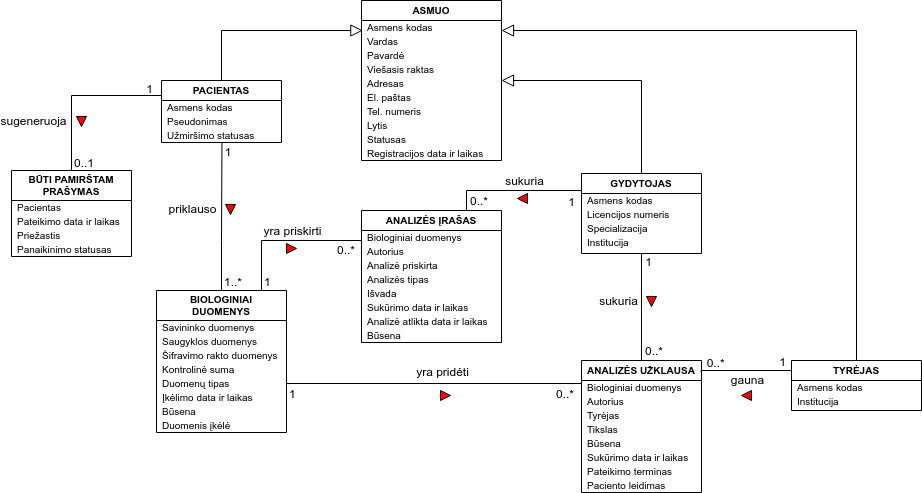
\includegraphics[width=1.05\linewidth]{ER.png}
        \vspace{-1\baselineskip}
        \caption{\small\textbf{Esybių - ryšių diagrama.}}
        \label{fig:image3}
    \end{center}
\end{figure}

\newpage

\subsubsection{Duomenų modelio specifikacija}
\noindent \textbf{E1: Esybė - \ttfamily ASMUO.} Generalizuojanti esybė, kuri
bendra visiems sistemos naudotojams (pacientams, gydytojams - genetikams,
tyrėjams).
\label{sec:E1}
\begin{table}[htb!]
    \small
    \captionsetup{justification=centering}
    \caption{\small\textbf{Esybės \texttt{ASMUO} specifikacija}.}
    \vskip -10pt
    \begin{tabular}{
        |>{\centering\arraybackslash}m{3cm}
        |>{\centering\arraybackslash}m{4.5cm}
        |>{\centering\arraybackslash}m{8.5cm}|
    }
        \hline
        \textbf{\cellcolor{deepchampagne}Atributas} &
        \textbf{\cellcolor{deepchampagne}Atributo apibūdinimas} &
        \textbf{\cellcolor{deepchampagne}Galimos reikšmės} \\
        \hline
        \multicolumn{1}{|>{\raggedright\ttfamily\arraybackslash}m{3cm}|}
            {Asmens kodas} &
        \multicolumn{1}{>{\raggedright\arraybackslash}m{4.5cm}|}{Unikalus
        asmeniui suteiktas identifikacinis numeris.} &
        \multicolumn{1}{>{\raggedright\arraybackslash}m{8.5cm}|}{
            Fiksuoto ilgio - 11 - skaitmenų kombinacija, kur:
            \begin{itemize}[leftmargin=0.5cm, itemsep=1pt, topsep=1pt,
                            after=\vspace{-1em}]
                \item \textbf{Pirmieji skaitmenys (1-6):} tai asmens gimimo
                data, užrašyta kaip „YYYYMMDD“ (metai, mėnuo, diena);
                \item \textbf{Septintasis skaitmuo:} tai ženklas, rodantis lytį.
                Jei skaitmuo yra nevedamas, tuomet jis rodo,
                kad žmogus yra vyriškos lyties (skaičius 1 arba 3), o jei
                moteriškos - (skaičius 2 arba 4);
                \item \textbf{Kiti skaitmenys (8-10):}  atsitiktinis numeris,
                skirtas užtikrinti, kad kiekvienas asmens kodas būtų unikalus;
                \item \textbf{11-asis skaitmuo:} tai kontrolinis skaitmuo,
                kurio paskirtis - patikrinti viso kodo tikslumą.
            \end{itemize}
        }
        \\
        \hline
        \multicolumn{1}{|>{\raggedright\ttfamily\arraybackslash}m{3cm}|}
            {Vardas} &
        \multicolumn{1}{>{\raggedright\arraybackslash}m{4.5cm}|}{Asmeniui
        suteiktas žodis, galintis padėti jį identifikuoti.} &
        \multicolumn{1}{>{\raggedright\arraybackslash}m{8.5cm}|}{Laisvas tekstas -
        raidžių kombinacija, kurią gali sudaryti iki 25 simbolių. Skaitmenys ir
        simboliai negali būti naudojami.} \\
        \hline
        \multicolumn{1}{|>{\raggedright\ttfamily\arraybackslash}m{3cm}|}
            {Pavardė} &
        \multicolumn{1}{>{\raggedright\arraybackslash}m{4.5cm}|}{Asmeniui
        suteiktas žodis, galintis padėti jį identifikuoti.} &
        \multicolumn{1}{>{\raggedright\arraybackslash}m{8.5cm}|}{Laisvas tekstas -
        raidžių kombinacija, kurią gali sudaryti iki 35 simbolių. Skaitmenys ir
        simboliai negali būti naudojami.} \\
        \hline
        \multicolumn{1}{|>{\raggedright\ttfamily\arraybackslash}m{3cm}|}
            {Viešasis raktas} &
        \multicolumn{1}{>{\raggedright\arraybackslash}m{4.5cm}|}{Vietoje, kurioje
        yra sistemos svečias, gali būti silpnas arba spartus internetas.} &
        \multicolumn{1}{>{\raggedright\arraybackslash}m{8.5cm}|}{Vietoje, kurioje
        yra sistemos svečias, gali būti silpnas arba spartus internetas.} \\
        \hline
        \multicolumn{1}{|>{\raggedright\ttfamily\arraybackslash}m{3cm}|}
            {Adresas} &
        \multicolumn{1}{>{\raggedright\arraybackslash}m{4.5cm}|}{Asmens gyvenamąją
        vietą apibūdinantis aprašymas.} & 
        \multicolumn{1}{>{\raggedright\arraybackslash}m{8.5cm}|}{Laisvas tekstas -
        raidžių kombinacija, kurią gali sudaryti iki 40 simbolių.} \\
        \hline
        \multicolumn{1}{|>{\raggedright\ttfamily\arraybackslash}m{3cm}|}
            {Elektroninis paštas} &
        \multicolumn{1}{>{\raggedright\arraybackslash}m{4.5cm}|}{Unikalus
        identifikatorius, kuriuo naudojantis galima susisiekti su tam tikru
        asmeniu.} &
        \multicolumn{1}{>{\raggedright\arraybackslash}m{8.5cm}|}{Laisvas tekstas -
        raidžių kombinacija, kurią gali sudaryti iki 50 simbolių. Simbolis
        '@' yra privalomas.}\\
        \hline
        \multicolumn{1}{|>{\raggedright\ttfamily\arraybackslash}m{3cm}|}
            {Telefono numeris} &
        \multicolumn{1}{>{\raggedright\arraybackslash}m{4.5cm}|}{Unikalus
        identifikatorius, kuriuo naudojantis galima susisiekti su tam tikru
        asmeniu.} &
        \multicolumn{1}{>{\raggedright\arraybackslash}m{8.5cm}|}{Fiksuoto ilgio
        (numatytas tik lietuviškų numerių naudojimas) - 12 - skaitmenų ir
        simbolių kombinacija (+370 6XX XXXXX), kur:
        \begin{itemize}[leftmargin=0.5cm, itemsep=1pt, topsep=1pt,
                        after=\vspace{-1em}]
            \item \textbf{+370:} šalies kodas;
            \item \textbf{6XX:} mobiliojo operatoriaus kodas;
            \item \textbf{XXXXX:} individualus numeris.
        \end{itemize}
        } \\
        \hline
        \multicolumn{1}{|>{\raggedright\ttfamily\arraybackslash}m{3cm}|}
            {Lytis} &
        \multicolumn{1}{>{\raggedright\arraybackslash}m{4.5cm}|}{Asmens
        biologinė lytis.} &
        \multicolumn{1}{>{\raggedright\arraybackslash}m{8.5cm}|}{\textbf{Galimos
        reikšmės:} vyras, moteris, kita.} \\
        \hline
        \multicolumn{1}{|>{\raggedright\ttfamily\arraybackslash}m{3cm}|}
            {Statusas} &
        \multicolumn{1}{>{\raggedright\arraybackslash}m{4.5cm}|}{Naudotojo
        paskyros būsena.} &
        \multicolumn{1}{>{\raggedright\arraybackslash}m{8.5cm}|}{\textbf{Galimos
        reikšmės:} aktyvus, archyvuotas, nebedirba.} \\
        \hline
    \end{tabular}
    \label{table:ER1_specifikacija}
\end{table}

\newpage

\label{sec:E1_2}
\begin{table}[htb!]
    \small
    \captionsetup{justification=centering}
    % \caption{\small\textbf{Esybės \texttt{ASMUO} specifikacija (tęsinys).}}
    \vskip -10pt
    \begin{tabular}{
        |>{\centering\arraybackslash}m{3cm}
        |>{\centering\arraybackslash}m{4.5cm}
        |>{\centering\arraybackslash}m{8.5cm}|
    }
        \hline
        \textbf{\cellcolor{deepchampagne}Atributas} &
        \textbf{\cellcolor{deepchampagne}Atributo apibūdinimas} &
        \textbf{\cellcolor{deepchampagne}Galimos reikšmės} \\
        \hline
        \multicolumn{1}{|>{\raggedright\ttfamily\arraybackslash}m{3cm}|}
            {Registracijos data ir laikas} &
        \multicolumn{1}{>{\raggedright\arraybackslash}m{4.5cm}|}{Reikšmė,
        nusakanti, kokiu metu (metai, mėnuo, diena, valandos, minutės, sekundės)
        buvo sukurta naudotojo paskyra.} &
        \multicolumn{1}{>{\raggedright\arraybackslash}m{8.5cm}|}{Užfiksuojama
        EINAMOJI\_DATA, kada buvo sukurta naudotojo paskyra. \textbf{Datos
        šablonas:} YYYY-MM-DD HH:MM, čia:
        \begin{itemize}[leftmargin=0.5cm, itemsep=1pt, topsep=1pt,
                        after=\vspace{-1em}]
            \item \textbf{YYYY:} metai;
            \item \textbf{MM:} mėnesis;
            \item \textbf{DD:} diena;
            \item \textbf{HH:} valandos;
            \item \textbf{MM:} minutės.
        \end{itemize}
        } \\
        \hline
    \end{tabular}
    \label{table:ER1_2specifikacija}
\end{table}

\newpage

\noindent \textbf{E2: Esybė - \ttfamily PACIENTAS.} Asmuo, kuris įkelia
biologinius duomenis ir valdo kitų asmenų prieigą prie šių duomenų.
\label{sec:E2}
\begin{table}[htb!]
    \captionsetup{justification=centering}
    \caption{\small\textbf{Esybės \texttt{PACIENTAS} specifikacija}.}
    \vskip -10pt
    \begin{tabular}{
        |>{\centering\arraybackslash}m{3cm}
        |>{\centering\arraybackslash}m{4.5cm}
        |>{\centering\arraybackslash}m{8.5cm}|
    }
        \hline
        \textbf{\cellcolor{deepchampagne}Atributas} &
        \textbf{\cellcolor{deepchampagne}Atributo apibūdinimas} &
        \textbf{\cellcolor{deepchampagne}Galimos reikšmės}  \\
        \hline
        \multicolumn{1}{|>{\raggedright\ttfamily\arraybackslash}m{3cm}|}
            {Asmens kodas} &
        \multicolumn{1}{>{\raggedright\arraybackslash}m{4.5cm}|}{Unikalus asmeniui
        suteiktas identifikacinis numeris.} &
        \multicolumn{1}{>{\raggedright\arraybackslash}m{8.5cm}|}{
            Fiksuoto ilgio - 11 - skaitmenų kombinacija, kur:
            \begin{itemize}[leftmargin=0.5cm, itemsep=1pt, topsep=1pt,
                            after=\vspace{-1em}]
                \item \textbf{Pirmieji skaitmenys (1-6):} tai asmens gimimo
                data, užrašyta kaip „YYYYMMDD“ (metai, mėnuo, diena);
                \item \textbf{Septintasis skaitmuo:} tai ženklas, rodantis lytį.
                Jei skaitmuo yra nevedamas, tuomet jis rodo,
                kad žmogus yra vyriškos lyties (skaičius 1 arba 3), o jei
                moteriškos - (skaičius 2 arba 4);
                \item \textbf{Kiti skaitmenys (8-10):}  atsitiktinis numeris,
                skirtas užtikrinti, kad kiekvienas asmens kodas būtų unikalus;
                \item \textbf{11-asis skaitmuo:} tai kontrolinis skaitmuo,
                kurio paskirtis - patikrinti viso kodo tikslumą.
            \end{itemize}
        }
        \\
        \hline
        \multicolumn{1}{|>{\raggedright\ttfamily\arraybackslash}m{3cm}|}
            {Pseudonimas} &
        \multicolumn{1}{>{\raggedright\arraybackslash}m{4.5cm}|}{Vietoje
        tikro naudotojo vardo naudojamas sugeneruotas raidžių, skaitmenų ir
        simbolių kombinacijos žodis.} &
        \multicolumn{1}{>{\raggedright\arraybackslash}m{8.5cm}|}{Laisvas
        tekstas - raidžių, skaitmenų ir simbolių kombinacija, kurią gali
        sudaryti iki 25 simbolių.}\\
        \hline
        \multicolumn{1}{|>{\raggedright\ttfamily\arraybackslash}m{3cm}|}
            {Užmiršimo statusas} &
        \multicolumn{1}{>{\raggedright\arraybackslash}m{4.5cm}|}{Požymis,
        nusakantis, ar naudotojas išreiškė norą, kad jo duomenys būtų
        ištrinti.} &
        \multicolumn{1}{>{\raggedright\arraybackslash}m{8.5cm}|}{\textbf{Galimos
        reikšmės:} 0 (noras neišreikštas) arba 1 (noras išreikštas).} \\
        \hline
    \end{tabular}
    \label{table:ER2_specifikacija}
\end{table}

\newpage

\noindent \textbf{E3: Esybė - \ttfamily GYDYTOJAS.} Asmuo, kuris kuria analizių
korteles bei teikia analizių užklausas tyrėjams.
\label{sec:E3}
\begin{table}[htb!]
    \captionsetup{justification=centering}
    \caption{\small\textbf{Esybės \texttt{GYDYTOJAS} specifikacija}.}
    \vskip -10pt
    \begin{tabular}{
        |>{\centering\arraybackslash}m{3cm}
        |>{\centering\arraybackslash}m{4.5cm}
        |>{\centering\arraybackslash}m{8.5cm}|
    }
        \hline
        \textbf{\cellcolor{deepchampagne}Atributas} &
        \textbf{\cellcolor{deepchampagne}Atributo apibūdinimas} &
        \textbf{\cellcolor{deepchampagne}Galimos reikšmės}  \\
        \hline
        \multicolumn{1}{|>{\raggedright\ttfamily\arraybackslash}m{3cm}|}
            {Asmens kodas} &
        \multicolumn{1}{>{\raggedright\arraybackslash}m{4.5cm}|}{Unikalus
        asmeniui suteiktas identifikacinis numeris.} &
        \multicolumn{1}{>{\raggedright\arraybackslash}m{8.5cm}|}{
            Fiksuoto ilgio - 11 - skaitmenų kombinacija, kur:
            \begin{itemize}[leftmargin=0.5cm, itemsep=1pt, topsep=1pt,
                            after=\vspace{-1em}]
                \item \textbf{Pirmieji skaitmenys (1-6):} tai asmens gimimo
                data, užrašyta kaip „YYYYMMDD“ (metai, mėnuo, diena);
                \item \textbf{Septintasis skaitmuo:} tai ženklas, rodantis lytį.
                Jei skaitmuo yra nevedamas, tuomet jis rodo,
                kad žmogus yra vyriškos lyties (skaičius 1 arba 3), o jei
                moteriškos - (skaičius 2 arba 4);
                \item \textbf{Kiti skaitmenys (8-10):}  atsitiktinis numeris,
                skirtas užtikrinti, kad kiekvienas asmens kodas būtų unikalus;
                \item \textbf{11-asis skaitmuo:} tai kontrolinis skaitmuo,
                kurio paskirtis - patikrinti viso kodo tikslumą.
            \end{itemize}
        }
        \\
        \hline
        \multicolumn{1}{|>{\raggedright\ttfamily\arraybackslash}m{3cm}|}
            {Licencijos numeris} &
        \multicolumn{1}{>{\raggedright\arraybackslash}m{4.5cm}|}{Unikalus
        tik gydytojams suteikiamas identifikacinis numeris.} &
        \multicolumn{1}{>{\raggedright\arraybackslash}m{8.5cm}|}{Fiksuoto
        ilgio - 6 - skaitmenų kombinacija.}\\
        \hline
        \multicolumn{1}{|>{\raggedright\ttfamily\arraybackslash}m{3cm}|}
            {Specializacija} &
        \multicolumn{1}{>{\raggedright\arraybackslash}m{4.5cm}|}{Medicinos
        sritis, kurioje gydytojas įgyja gilų žinių ir įgūdžių lygį, kad galėtų
        gydyti tam tikras ligas.} &
        \multicolumn{1}{>{\raggedright\arraybackslash}m{8.5cm}|}{Laisvas
        tekstas - raidžių kombinacija, kurią gali sudaryti iki 40 simbolių.} \\
        \hline
        \multicolumn{1}{|>{\raggedright\ttfamily\arraybackslash}m{3cm}|}
            {Institucija} &
        \multicolumn{1}{>{\raggedright\arraybackslash}m{4.5cm}|}{Įstaigos,
        kurioje dirba gydytojas, pavadinimas ir adresas.} &
        \multicolumn{1}{>{\raggedright\arraybackslash}m{8.5cm}|}{Laisvas
        tekstas - raidžių kombinacija, kurią gali sudaryti iki 70 simbolių.} \\
        \hline
    \end{tabular}
    \label{table:ER3_specifikacija}
\end{table}

\newpage

\noindent \textbf{E4: Esybė - \ttfamily TYRĖJAS.} Asmuo, kuris atlieka
biologinių duomenų analizę ir teikia išvadas gydytojui - genetikui.
\label{sec:E4}
\begin{table}[htb!]
    \captionsetup{justification=centering}
    \caption{\small\textbf{Esybės \texttt{TYRĖJAS} specifikacija}.}
    \vskip -10pt
    \begin{tabular}{
        |>{\centering\arraybackslash}m{3cm}
        |>{\centering\arraybackslash}m{4.5cm}
        |>{\centering\arraybackslash}m{8.5cm}|
    }
        \hline
        \textbf{\cellcolor{deepchampagne}Atributas} &
        \textbf{\cellcolor{deepchampagne}Atributo apibūdinimas} &
        \textbf{\cellcolor{deepchampagne}Galimos reikšmės}  \\
        \hline
        \multicolumn{1}{|>{\raggedright\ttfamily\arraybackslash}m{3cm}|}
            {Asmens kodas} &
        \multicolumn{1}{>{\raggedright\arraybackslash}m{4.5cm}|}{Unikalus
        asmeniui suteiktas identifikacinis numeris.} &
        \multicolumn{1}{>{\raggedright\arraybackslash}m{8.5cm}|}{
            Fiksuoto ilgio - 11 - skaitmenų kombinacija, kur:
            \begin{itemize}[leftmargin=0.5cm, itemsep=1pt, topsep=1pt,
                            after=\vspace{-1em}]
                \item \textbf{Pirmieji skaitmenys (1-6):} tai asmens gimimo
                data, užrašyta kaip „YYYYMMDD“ (metai, mėnuo, diena);
                \item \textbf{Septintasis skaitmuo:} tai ženklas, rodantis lytį.
                Jei skaitmuo yra nevedamas, tuomet jis rodo,
                kad žmogus yra vyriškos lyties (skaičius 1 arba 3), o jei
                moteriškos - (skaičius 2 arba 4);
                \item \textbf{Kiti skaitmenys (8-10):}  atsitiktinis numeris,
                skirtas užtikrinti, kad kiekvienas asmens kodas būtų unikalus;
                \item \textbf{11-asis skaitmuo:} tai kontrolinis skaitmuo,
                kurio paskirtis - patikrinti viso kodo tikslumą.
            \end{itemize}
        }
        \\
        \hline
        \multicolumn{1}{|>{\raggedright\ttfamily\arraybackslash}m{3cm}|}
            {Institucija} &
        \multicolumn{1}{>{\raggedright\arraybackslash}m{4.5cm}|}{Įstaigos,
        kurioje dirba tyrėjas, pavadinimas ir adresas.} &
        \multicolumn{1}{>{\raggedright\arraybackslash}m{8.5cm}|}{Laisvas
        tekstas - raidžių kombinacija, kurią gali sudaryti iki 70 simbolių.} \\
        \hline
    \end{tabular}
    \label{table:ER4_specifikacija}
\end{table}

\newpage

\noindent \textbf{E5: Esybė - \ttfamily BŪTI PAMIRŠTAM PRAŠYMAS.} Prašymas,
kuris yra sugeneruojamas paciento, norinčio, kad jo duomenys būtų panaikinti iš
sistemos.
\label{sec:E5}
\begin{table}[htb!]
    \captionsetup{justification=centering}
    \caption{\small\textbf{Esybės \texttt{BŪTI PAMIRŠTAM PRAŠYMAS}
    specifikacija}.}
    \vskip -10pt
    \begin{tabular}{
        |>{\centering\arraybackslash}m{3cm}
        |>{\centering\arraybackslash}m{4.5cm}
        |>{\centering\arraybackslash}m{8.5cm}|
    }
        \hline
        \textbf{\cellcolor{deepchampagne}Atributas} &
        \textbf{\cellcolor{deepchampagne}Atributo apibūdinimas} &
        \textbf{\cellcolor{deepchampagne}Galimos reikšmės}  \\
        \hline
        \multicolumn{1}{|>{\raggedright\ttfamily\arraybackslash}m{3cm}|}
            {Pacientas} &
        \multicolumn{1}{>{\raggedright\arraybackslash}m{4.5cm}|}{Unikalus
        pacientą identifikuojantis numeris.} &
        \multicolumn{1}{>{\raggedright\arraybackslash}m{8.5cm}|}{Nefiksuoto
        ilgio skaitmenų kombinacija.}\\
        \hline
        \multicolumn{1}{|>{\raggedright\ttfamily\arraybackslash}m{3cm}|}
            {Pateikimo data ir laikas} &
            \multicolumn{1}{>{\raggedright\arraybackslash}m{4.5cm}|}{Reikšmė,
            nusakanti, kokiu metu (metai, mėnuo, diena, valandos, minutės,
            sekundės) buvo pateikta užklausa „būti pamirštam“.} &
            \multicolumn{1}{>{\raggedright\arraybackslash}m{8.5cm}|}{
                Užfiksuojama EINAMOJI\_DATA, kada buvo pateikta užklausa.
                \textbf{Datos šablonas:} YYYY-MM-DD HH:MM, čia:
                \begin{itemize}[leftmargin=0.5cm, itemsep=1pt, topsep=1pt,
                                after=\vspace{-1em}]
                    \item \textbf{YYYY:} metai;
                    \item \textbf{MM:} mėnesis;
                    \item \textbf{DD:} diena;
                    \item \textbf{HH:} valandos;
                    \item \textbf{MM:} minutės.
                \end{itemize}
            } \\
        \hline
        \multicolumn{1}{|>{\raggedright\ttfamily\arraybackslash}m{3cm}|}
            {Priežastis} &
        \multicolumn{1}{>{\raggedright\arraybackslash}m{4.5cm}|}{Paaiškinimas,
        kodėl naudotojas nori, kad jo duomenys būtų panaikinti iš saugyklų.} &
        \multicolumn{1}{>{\raggedright\arraybackslash}m{8.5cm}|}{Laisvas
        tekstas - raidžių kombinacija, kurią gali sudaryti iki 50 simbolių.}\\
        \hline
        \multicolumn{1}{|>{\raggedright\ttfamily\arraybackslash}m{3cm}|}
            {Panaikinimo statusas} &
        \multicolumn{1}{>{\raggedright\arraybackslash}m{4.5cm}|}{Požymis,
        nusakantis, ar naudotojo duomenys buvo panaikinti.} &
        \multicolumn{1}{>{\raggedright\arraybackslash}m{8.5cm}|}{\textbf{Galimos
        reikšmės:} 0 (duomenys nepanaikinti) arba 1 (duomenys panaikinti).} \\
        \hline
    \end{tabular}
    \label{table:ER5_specifikacija}
\end{table}

\newpage

\noindent \textbf{E6: Esybė - \ttfamily BIOLOGINIAI DUOMENYS.} Struktūrizuota
informacija apie biologinius duomenis, kuriuos pacientas įkelia į sistemą.
\label{sec:E6}
\begin{table}[htb!]
    \captionsetup{justification=centering}
    \caption{\small\textbf{Esybės \texttt{BIOLOGINIAI DUOMENYS}
    specifikacija}.}
    \vskip -10pt
    \begin{tabular}{
        |>{\centering\arraybackslash}m{3cm}
        |>{\centering\arraybackslash}m{4.5cm}
        |>{\centering\arraybackslash}m{8.5cm}|
    }
        \hline
        \textbf{\cellcolor{deepchampagne}Atributas} &
        \textbf{\cellcolor{deepchampagne}Atributo apibūdinimas} &
        \textbf{\cellcolor{deepchampagne}Galimos reikšmės}  \\
        \hline
        \multicolumn{1}{|>{\raggedright\ttfamily\arraybackslash}m{3cm}|}
            {Savininko duomenys} &
        \multicolumn{1}{>{\raggedright\arraybackslash}m{4.5cm}|}{Unikalus
        pseudonimizuotas paciento identifikatorius.} &
        \multicolumn{1}{>{\raggedright\arraybackslash}m{8.5cm}|}{Nefiksuoto
        ilgio skaitmenų kombinacija.}\\
        \hline
        \multicolumn{1}{|>{\raggedright\ttfamily\arraybackslash}m{3cm}|}
            {Saugyklos duomenys} &
        \multicolumn{1}{>{\raggedright\arraybackslash}m{4.5cm}|}{Nuoroda į
        šifruotą failą.} &
        \multicolumn{1}{>{\raggedright\arraybackslash}m{8.5cm}|}{Nefiksuoto
        ilgio simbolių kombinacija.}\\
        \hline
        \multicolumn{1}{|>{\raggedright\ttfamily\arraybackslash}m{3cm}|}
            {Šifravimo rakto duomenys} &
        \multicolumn{1}{>{\raggedright\arraybackslash}m{4.5cm}|}{Nuoroda į
        raktą, su kuriuo buvo užšifruoti biologiniai duomenys.} &
        \multicolumn{1}{>{\raggedright\arraybackslash}m{8.5cm}|}{Nefiksuoto
        ilgio simbolių kombinacija.}\\
        \hline
        \multicolumn{1}{|>{\raggedright\ttfamily\arraybackslash}m{3cm}|}
            {Kontrolinė suma} &
        \multicolumn{1}{>{\raggedright\arraybackslash}m{4.5cm}|}{Reikšmė,
        leidžianti patikrinti duomenų vientisumą.} &
        \multicolumn{1}{>{\raggedright\arraybackslash}m{8.5cm}|}{Nefiksuoto
        ilgio skaitmenų kombinacija.}\\
        \hline
        \multicolumn{1}{|>{\raggedright\ttfamily\arraybackslash}m{3cm}|}
            {Duomenų tipas} &
        \multicolumn{1}{>{\raggedright\arraybackslash}m{4.5cm}|}{Įkelto
        biologinių duomenų failo apibūdinimas} &
        \multicolumn{1}{>{\raggedright\arraybackslash}m{8.5cm}|}{Laisvas
        tekstas - raidžių kombinacija, kurią gali sudaryti iki 50 simbolių.}\\
        \hline
        \multicolumn{1}{|>{\raggedright\ttfamily\arraybackslash}m{3cm}|}
            {Įkėlimo data ir laikas} &
        \multicolumn{1}{>{\raggedright\arraybackslash}m{4.5cm}|}{Reikšmė,
        nusakanti, kokiu metu (metai, mėnuo, diena, valandos, minutės, sekundės)
        buvo įkeltas biologinių duomenų failas.} &
        \multicolumn{1}{>{\raggedright\arraybackslash}m{8.5cm}|}{Užfiksuojama
        EINAMOJI\_DATA, kada buvo įkelti duomenys. \textbf{Datos
        šablonas:} YYYY-MM-DD HH:MM, čia:
        \begin{itemize}[leftmargin=0.5cm, itemsep=1pt, topsep=1pt,
                        after=\vspace{-1em}]
            \item \textbf{YYYY:} metai;
            \item \textbf{MM:} mėnesis;
            \item \textbf{DD:} diena;
            \item \textbf{HH:} valandos;
            \item \textbf{MM:} minutės.
        \end{itemize}
        } \\
        \hline
        \multicolumn{1}{|>{\raggedright\ttfamily\arraybackslash}m{3cm}|}
            {Būsena} &
        \multicolumn{1}{>{\raggedright\arraybackslash}m{4.5cm}|}{Biologinių
        duomenų analizės vykdymo būsena} &
        \multicolumn{1}{>{\raggedright\arraybackslash}m{8.5cm}|}{\textbf{Galimos
        reikšmės:} laukiama, analizuojama, užbaigta, atmesta.} \\
        \hline
        \multicolumn{1}{|>{\raggedright\ttfamily\arraybackslash}m{3cm}|}
            {Duomenis įkėlė} &
        \multicolumn{1}{>{\raggedright\arraybackslash}m{4.5cm}|}{Unikalus
        gydytoją identifikuojantis numeris.} &
        \multicolumn{1}{>{\raggedright\arraybackslash}m{8.5cm}|}{Nefiksuoto
        ilgio skaitmenų kombinacija.} \\
        \hline
    \end{tabular}
    \label{table:ER6_specifikacija}
\end{table}

\newpage

\noindent \textbf{E7: Esybė - \ttfamily ANALIZĖS ĮRAŠAS.}
Struktūrizuota informacija apie atliktą biologinių duomenų analizę (analizės
tipą ir išvadas).
\label{sec:E7}
\begin{table}[htb!]
    \captionsetup{justification=centering}
    \caption{\small\textbf{Esybės \texttt{ANALIZĖS ĮRAŠAS}
    specifikacija}.}
    \vskip -10pt
    \begin{tabular}{
        |>{\centering\arraybackslash}m{3cm}
        |>{\centering\arraybackslash}m{4.5cm}
        |>{\centering\arraybackslash}m{8.5cm}|
    }
        \hline
        \textbf{\cellcolor{deepchampagne}Atributas} &
        \textbf{\cellcolor{deepchampagne}Atributo apibūdinimas} &
        \textbf{\cellcolor{deepchampagne}Galimos reikšmės}  \\
        \hline
        \multicolumn{1}{|>{\raggedright\ttfamily\arraybackslash}m{3cm}|}
            {Biologiniai duomenys} &
        \multicolumn{1}{>{\raggedright\arraybackslash}m{4.5cm}|}{Unikalus
        biologinius duomenis identifikuojantis numeris.} &
        \multicolumn{1}{>{\raggedright\arraybackslash}m{8.5cm}|}{Nefiksuoto
        ilgio skaitmenų kombinacija.}\\
        \hline
        \multicolumn{1}{|>{\raggedright\ttfamily\arraybackslash}m{3cm}|}
            {Autorius} &
        \multicolumn{1}{>{\raggedright\arraybackslash}m{4.5cm}|}{Unikalus
        gydytoją identifikuojantis numeris.} &
        \multicolumn{1}{>{\raggedright\arraybackslash}m{8.5cm}|}{Nefiksuoto
        ilgio skaitmenų kombinacija.}\\
        \hline
        \multicolumn{1}{|>{\raggedright\ttfamily\arraybackslash}m{3cm}|}
            {Analizė priskirta} &
        \multicolumn{1}{>{\raggedright\arraybackslash}m{4.5cm}|}{Unikalus
        tyrėją identifikuojantis numeris.} &
        \multicolumn{1}{>{\raggedright\arraybackslash}m{8.5cm}|}{Nefiksuoto
        ilgio skaitmenų kombinacija.}\\
        \hline
        \multicolumn{1}{|>{\raggedright\ttfamily\arraybackslash}m{3cm}|}
            {Analizės tipas} &
        \multicolumn{1}{>{\raggedright\arraybackslash}m{4.5cm}|}{Apibūdinimas,
        kokiu būdu yra analizuojami įkelti biologiniai duomenys.} &
        \multicolumn{1}{>{\raggedright\arraybackslash}m{8.5cm}|}{Laisvas
        tekstas - raidžių kombinacija, kurią gali sudaryti iki 30 simbolių.}\\
        \hline
        \multicolumn{1}{|>{\raggedright\ttfamily\arraybackslash}m{3cm}|}
            {Išvada} &
        \multicolumn{1}{>{\raggedright\arraybackslash}m{4.5cm}|}{Atliktos
        biologinių duomenų analizės rezultatas.} &
        \multicolumn{1}{>{\raggedright\arraybackslash}m{8.5cm}|}{Laisvas
        tekstas - raidžių kombinacija, kurią gali sudaryti iki 100 simbolių.} \\
        \hline
        \multicolumn{1}{|>{\raggedright\ttfamily\arraybackslash}m{3cm}|}
            {Sukūrimo data ir laikas} &
            \multicolumn{1}{>{\raggedright\arraybackslash}m{4.5cm}|}{Reikšmė,
            nusakanti, kokiu metu (metai, mėnuo, diena, valandos, minutės,
            sekundės) buvo sukurtas analizės įrašas.} &
            \multicolumn{1}{>{\raggedright\arraybackslash}m{8.5cm}|}{
                Užfiksuojama analizės įrašo sukūrimo data ir laikas.
                \textbf{Datos šablonas:} YYYY-MM-DD HH:MM, čia:
                \begin{itemize}[leftmargin=0.5cm, itemsep=1pt, topsep=1pt,
                                after=\vspace{-1em}]
                    \item \textbf{YYYY:} metai;
                    \item \textbf{MM:} mėnesis;
                    \item \textbf{DD:} diena;
                    \item \textbf{HH:} valandos;
                    \item \textbf{MM:} minutės.
                \end{itemize}
            } \\
        \hline
        \multicolumn{1}{|>{\raggedright\ttfamily\arraybackslash}m{3cm}|}
            {Analizė atlikta data ir laikas} &
            \multicolumn{1}{>{\raggedright\arraybackslash}m{4.5cm}|}{Reikšmė,
            nusakanti, kokiu metu (metai, mėnuo, diena, valandos, minutės,
            sekundės) buvo atlikta analizė.} &
            \multicolumn{1}{>{\raggedright\arraybackslash}m{8.5cm}|}{
                Užfiksuojama analizės atlikimo data ir laikas.
                \textbf{Datos šablonas:} YYYY-MM-DD HH:MM, čia:
                \begin{itemize}[leftmargin=0.5cm, itemsep=1pt, topsep=1pt,
                                after=\vspace{-1em}]
                    \item \textbf{YYYY:} metai;
                    \item \textbf{MM:} mėnesis;
                    \item \textbf{DD:} diena;
                    \item \textbf{HH:} valandos;
                    \item \textbf{MM:} minutės.
                \end{itemize}
            } \\
        \hline
        \multicolumn{1}{|>{\raggedright\ttfamily\arraybackslash}m{3cm}|}
            {Būsena} &
        \multicolumn{1}{>{\raggedright\arraybackslash}m{4.5cm}|}{Biologinių
        duomenų analizės vykdymo būsena.} &
        \multicolumn{1}{>{\raggedright\arraybackslash}m{8.5cm}|}{\textbf{Galimos
        reikšmės:} laukiama, analizuojama, užbaigta, atmesta.}\\
        \hline
    \end{tabular}
    \label{table:ER7_specifikacija}
\end{table}

\newpage

\noindent \textbf{E8: Esybė - \ttfamily ANALIZĖS UŽKLAUSA.}
Struktūrizuota informacija apie reikalingą biologinių duomeų analizę, kuri yra
siunčiama tyrėjams.
\label{sec:E8}
\begin{table}[htb!]
    \captionsetup{justification=centering}
    \caption{\small\textbf{Esybės \texttt{ANALIZĖS UŽKLAUSA}
    specifikacija}.}
    \vskip -10pt
    \begin{tabular}{
        |>{\centering\arraybackslash}m{3cm}
        |>{\centering\arraybackslash}m{4.5cm}
        |>{\centering\arraybackslash}m{8.5cm}|
    }
        \hline
        \textbf{\cellcolor{deepchampagne}Atributas} &
        \textbf{\cellcolor{deepchampagne}Atributo apibūdinimas} &
        \textbf{\cellcolor{deepchampagne}Galimos reikšmės}  \\
        \hline
        \multicolumn{1}{|>{\raggedright\ttfamily\arraybackslash}m{3cm}|}
            {Biologiniai duomenys} &
        \multicolumn{1}{>{\raggedright\arraybackslash}m{4.5cm}|}{Unikalus
        biologinius duomenis identifikuojantis numeris.} &
        \multicolumn{1}{>{\raggedright\arraybackslash}m{8.5cm}|}{Nefiksuoto
        ilgio skaitmenų kombinacija.}\\
        \hline
        \multicolumn{1}{|>{\raggedright\ttfamily\arraybackslash}m{3cm}|}
            {Autorius} &
        \multicolumn{1}{>{\raggedright\arraybackslash}m{4.5cm}|}{Unikalus
        gydytoją identifikuojantis numeris.} &
        \multicolumn{1}{>{\raggedright\arraybackslash}m{8.5cm}|}{Nefiksuoto
        ilgio skaitmenų kombinacija.}\\
        \hline
        \multicolumn{1}{|>{\raggedright\ttfamily\arraybackslash}m{3cm}|}
            {Tyrėjas} &
        \multicolumn{1}{>{\raggedright\arraybackslash}m{4.5cm}|}{Unikalus
        tyrėją identifikuojantis numeris.} &
        \multicolumn{1}{>{\raggedright\arraybackslash}m{8.5cm}|}{Nefiksuoto
        ilgio skaitmenų kombinacija.}\\
        \hline
        \multicolumn{1}{|>{\raggedright\ttfamily\arraybackslash}m{3cm}|}
            {Tikslas} &
        \multicolumn{1}{>{\raggedright\arraybackslash}m{4.5cm}|}{Apibūdinimas,
        koks yra reikalingos analizės tikslas.} &
        \multicolumn{1}{>{\raggedright\arraybackslash}m{8.5cm}|}{Laisvas
        tekstas - raidžių kombinacija, kurią gali sudaryti iki 50 simbolių.}\\
        \hline
        \multicolumn{1}{|>{\raggedright\ttfamily\arraybackslash}m{3cm}|}
            {Būsena} &
        \multicolumn{1}{>{\raggedright\arraybackslash}m{4.5cm}|}{Biologinių
        duomenų analizės vykdymo būsena.} &
        \multicolumn{1}{>{\raggedright\arraybackslash}m{8.5cm}|}{\textbf{Galimos
        reikšmės:} laukiama, analizuojama, užbaigta, atmesta.}\\
        \hline
        \multicolumn{1}{|>{\raggedright\ttfamily\arraybackslash}m{3cm}|}
            {Sukūrimo data ir laikas} &
            \multicolumn{1}{>{\raggedright\arraybackslash}m{4.5cm}|}{Reikšmė,
            nusakanti, kokiu metu (metai, mėnuo, diena, valandos, minutės,
            sekundės) buvo sukurta užklausa tyrėjui.} &
            \multicolumn{1}{>{\raggedright\arraybackslash}m{8.5cm}|}{
                Užfiksuojama analizės užklausos sukūrimo data ir laikas.
                \textbf{Datos šablonas:} YYYY-MM-DD HH:MM, čia:
                \begin{itemize}[leftmargin=0.5cm, itemsep=1pt, topsep=1pt,
                                after=\vspace{-1em}]
                    \item \textbf{YYYY:} metai;
                    \item \textbf{MM:} mėnesis;
                    \item \textbf{DD:} diena;
                    \item \textbf{HH:} valandos;
                    \item \textbf{MM:} minutės.
                \end{itemize}
            } \\
        \hline
        \multicolumn{1}{|>{\raggedright\ttfamily\arraybackslash}m{3cm}|}
            {Pateikimo terminas} &
            \multicolumn{1}{>{\raggedright\arraybackslash}m{4.5cm}|}{Reikšmė,
            nusakanti, iki kada (metai, mėnuo, diena, valandos, minutės,
            sekundės) turi būti atlikta analizė.} &
            \multicolumn{1}{>{\raggedright\arraybackslash}m{8.5cm}|}{
                Nurodomas analizės atlikimo terminas.
                \textbf{Datos šablonas:} YYYY-MM-DD HH:MM, čia:
                \begin{itemize}[leftmargin=0.5cm, itemsep=1pt, topsep=1pt,
                                after=\vspace{-1em}]
                    \item \textbf{YYYY:} metai;
                    \item \textbf{MM:} mėnesis;
                    \item \textbf{DD:} diena;
                    \item \textbf{HH:} valandos;
                    \item \textbf{MM:} minutės.
                \end{itemize}
            } \\
        \hline
        \multicolumn{1}{|>{\raggedright\ttfamily\arraybackslash}m{3cm}|}
            {Paciento leidimas} &
        \multicolumn{1}{>{\raggedright\arraybackslash}m{4.5cm}|}{Požymis,
        nusakantis, ar naudotojas davė leidimą vykdyti analizę su jo pateiktais
        duomenimis.} &
        \multicolumn{1}{>{\raggedright\arraybackslash}m{8.5cm}|}{\textbf{Galimos
        reikšmės:} 0 (leidimas negautas) arba 1 (leidimas gautas).}\\
        \hline
    \end{tabular}
    \label{table:ER8_specifikacija}
\end{table}

\newpage

\section{Reikalavimai sistemos išvaizdai}
Kuriant savarankiškos suverenios pseudonimizuotos tapatybės valdymo sistemą
turi būti laikomąsi žemiau aprašytų sistemos išvaizdos reikalavimų.
\vskip 10pt

\noindent \textbf{NF1:} Sistemos sąsaja turi būti neįkyri.
\label{sec:NF1}
\begin{table}[htb!]
    \captionsetup{justification=centering}
    \begin{tabular}{|m{4.9cm}|m{11cm}|}
        \hline
        \raggedleft \textbf{\cellcolor{deepchampagne}Pagrindimas} &
        Sisteminiuose languose neturi būti realizuoti iššokantys modaliniai
        langeliai, kuriuose reikia pasirinkti, ar tikrai norima išsaugoti
        įvestus duomenis. \\
        \hline
        \raggedleft \textbf{\cellcolor{deepchampagne}Šaltinis} & Užsakovas. \\
        \hline
        \raggedleft \textbf{\cellcolor{deepchampagne}Atitikimo kriterijus} & 
        Užpildžius duomenų įvedimo formas ir išsaugojus duomenis nepasirodo
        iššokantis modalinis langelis su pranešimu apie reikalingą duomenų
        įvedimo patvirtinimą - duomenys yra išsaugomi be papildomo naudotojo
        veiksmo. \\
        \hline
        \raggedleft \textbf{\cellcolor{deepchampagne}Užsakovo tenkinimas} & 1. \\
        \hline
        \raggedleft \textbf{\cellcolor{deepchampagne}Užsakovo netenkinimas} & 3. \\
        \hline
        \raggedleft \textbf{\cellcolor{deepchampagne}Prioritetas} & Vidutinis. \\
        \hline
        \raggedleft \textbf{\cellcolor{deepchampagne}Konfliktai} & Nėra. \\
        \hline
    \end{tabular}
\end{table}

\noindent \textbf{NF2:} Sistema turi būti pritaikyta darbui įvairaus amžiaus
žmonėms.
\label{sec:NF2}
\begin{table}[htb!]
    \captionsetup{justification=centering}
    \begin{tabular}{|m{4.9cm}|m{11cm}|}
        \hline
        \raggedleft \textbf{\cellcolor{deepchampagne}Pagrindimas} &
        Sistema gali naudotis įvairaus amžiaus asmenys (sistemos svečiai,
        registruoti naudotojai: gydytojai - genetikai, tyrėjai), kurie dėl savo
        amžiaus gali turėti regėjimo sutrikimų, todėl sistemoje turi būti galima
        keisti langų mastelį, neišdarkant sistemos langus sudarančių elementų
        išdėstymo ir nepakenkiant naudotojo naudojimo sistema patirčiai. \\
        \hline
        \raggedleft \textbf{\cellcolor{deepchampagne}Šaltinis} & Užsakovas. \\
        \hline
        \raggedleft \textbf{\cellcolor{deepchampagne}Atitikimo kriterijus} & 
        Sistemos naudotojai, pakeitę mastelį, gali ir toliau sėkmingai naudotis
        sistemos funkcionalumu ir matyti sistemos langus sudarančius elementus
        (nesukeliant naudotojų susierzinimo) dėl sistemos gebėjimo prisitaikyti
        prie keičiamo mastelio. \\
        \hline
        \raggedleft \textbf{\cellcolor{deepchampagne}Užsakovo tenkinimas} & 1. \\
        \hline
        \raggedleft \textbf{\cellcolor{deepchampagne}Užsakovo netenkinimas} & 3. \\
        \hline
        \raggedleft \textbf{\cellcolor{deepchampagne}Prioritetas} & Aukštas. \\
        \hline
        \raggedleft \textbf{\cellcolor{deepchampagne}Konfliktai} & Nėra. \\
        \hline
    \end{tabular}
\end{table}

\newpage

\noindent \textbf{NF3:} Sistema turi būti intuityvi.
\label{sec:NF3}
\begin{table}[htb!]
    \captionsetup{justification=centering}
    \begin{tabular}{|m{4.9cm}|m{11cm}|}
        \hline
        \raggedleft \textbf{\cellcolor{deepchampagne}Pagrindimas} &
        Sistema gali naudotis įvairaus amžiaus asmenys, turintys nevienodą
        technologinio raštingumo bei išsilavinimo lygį, todėl sistemos languose
        turi būti naudojami nedviprasmiški ir plačiai visuomenės asmenų daliai
        suprantami sistemos meniu juostos pasirinkimų pavadinimai bei turi būti
        panaudota kuo mažiau kompleksinių informacijos pateikimo struktūrų
        (pavyzdžiui, medžio struktūrų). \\
        \hline
        \raggedleft \textbf{\cellcolor{deepchampagne}Šaltinis} & Užsakovas. \\
        \hline
        \raggedleft \textbf{\cellcolor{deepchampagne}Atitikimo kriterijus} & 
        Jeigu įvykdžius visų sistemos naudotojų apklausą praėjus 2 mėn. po
        sistemos eksploatavimo pradžios nesulaukta daugiau
        nei 10\% atsiliepimų dėl sistemos neintuityvumo, nefunkcinis
        reikalavimas įgyvendintas. \\
        \hline
        \raggedleft \textbf{\cellcolor{deepchampagne}Užsakovo tenkinimas} & 1. \\
        \hline
        \raggedleft \textbf{\cellcolor{deepchampagne}Užsakovo netenkinimas} & 4. \\
        \hline
        \raggedleft \textbf{\cellcolor{deepchampagne}Prioritetas} & Aukštas. \\
        \hline
        \raggedleft \textbf{\cellcolor{deepchampagne}Konfliktai} & Nėra. \\
        \hline
    \end{tabular}
\end{table}

\newpage

\section{Reikalavimai panaudojamumui}
Kuriant savarankiškos suverenios pseudonimizuotos tapatybės valdymo sistemą
turi būti laikomąsi žemiau aprašytų panaudojamumo reikalavimų.
\vskip 10pt

\noindent \textbf{NF4:} Sistema turi būti nesudėtinga naudotis sistemos
naudotojams.
\label{sec:NF4}
\begin{table}[htb!]
    \captionsetup{justification=centering}
    \vskip -10pt
    \begin{tabular}{|m{4.9cm}|m{11cm}|}
        \hline
        \raggedleft \textbf{\cellcolor{deepchampagne}Pagrindimas} &
        Sistema gali naudotis įvairaus amžiaus bei skirtingo išsilavinimo lygio
        asmenys, todėl sistemos naudotojai turi sugebėti tinkamai naudotis
        sistemos funkcionalumais ir užpildyti sistemoje prieinamas formas be
        papildomų mokymų (turi būti pateikiami detalūs funkcionalumų aprašymai;
        pildant sistemos formas turi būti pateikiami aiškūs ir išsamūs
        paaiškinimai, kokia informacija turi būti įvesta kiekviename lauke). \\
        \hline
        \raggedleft \textbf{\cellcolor{deepchampagne}Šaltinis} & Užsakovas. \\
        \hline
        \raggedleft \textbf{\cellcolor{deepchampagne}Atitikimo kriterijus} & 
        Jeigu įvykdžius sistemos naudotojų apklausą praėjus 2 mėn. po sistemos
        eksploatavimo pradžios nesulaukta nei vieno atsiliepimo dėl sudėtingo
        sistemos naudojimo, nefunkcinis reikalavimas įgyvendintas. \\
        \hline
        \raggedleft \textbf{\cellcolor{deepchampagne}Užsakovo tenkinimas} & 2. \\
        \hline
        \raggedleft \textbf{\cellcolor{deepchampagne}Užsakovo netenkinimas} & 2. \\
        \hline
        \raggedleft \textbf{\cellcolor{deepchampagne}Prioritetas} & Aukštas. \\
        \hline
        \raggedleft \textbf{\cellcolor{deepchampagne}Konfliktai} & Nėra. \\
        \hline
    \end{tabular}
\end{table}

\noindent \textbf{NF5:} Turi būti suteikta galimybė visiems sistemos naudotojams
suprasti sistemoje naudojamus terminus.
\label{sec:NF5}
\begin{table}[htb!]
    \captionsetup{justification=centering}
    \vskip -10pt
    \begin{tabular}{|m{4.9cm}|m{11cm}|}
        \hline
        \raggedleft \textbf{\cellcolor{deepchampagne}Pagrindimas} &
        Sistemoje pateikta informacija turi būti parašyta taip, jog būtų
        suprantama ne tik medicininės dalykinės srities ekspertams. Šalia
        kiekvieno naudojamo medicininio termino turi būti pridėta nuoroda,
        nukreipianti į sistemos langą, kuriame pateiktas techninių terminų
        žodynas. \\
        \hline
        \raggedleft \textbf{\cellcolor{deepchampagne}Šaltinis} & Užsakovas. \\
        \hline
        \raggedleft \textbf{\cellcolor{deepchampagne}Atitikimo kriterijus} & 
        Jeigu įvykdžius sistemos naudotojų apklausą praėjus 2 mėn. po sistemos
        eksploatavimo pradžios nesulaukta nei vieno atsiliepimo dėl sudėtingo
        sistemos naudojimo, nefunkcinis reikalavimas įgyvendintas. \\
        \hline
        \raggedleft \textbf{\cellcolor{deepchampagne}Užsakovo tenkinimas} & 2. \\
        \hline
        \raggedleft \textbf{\cellcolor{deepchampagne}Užsakovo netenkinimas} & 2. \\
        \hline
        \raggedleft \textbf{\cellcolor{deepchampagne}Prioritetas} & Žemas. \\
        \hline
        \raggedleft \textbf{\cellcolor{deepchampagne}Konfliktai} & Nėra. \\
        \hline
    \end{tabular}
\end{table}

\newpage

\section{Reikalavimai vykdymo charakteristikoms}
Kuriant savarankiškos suverenios pseudonimizuotos tapatybės valdymo sistemą
turi būti laikomąsi žemiau aprašytų vykdymo charakteristikų reikalavimų.
\vskip 10pt

\noindent \textbf{NF6:} Autentifikacijos (tapatybės patikrinimo) operacija turi
būti įvykdyta per < 1 s.
\label{sec:NF6}
\begin{table}[htb!]
    \captionsetup{justification=centering}
    \vskip -10pt
    \begin{tabular}{|m{4.9cm}|m{11cm}|}
        \hline
        \raggedleft \textbf{\cellcolor{deepchampagne}Pagrindimas} &
        Greitas autentifikacijos procesas suteikia didesnį naudotojų
        pasitikėjimą sistema bei padeda užtikrinti po autentifikacijos sekančių
        operacijų atlikimą numatytu laiku. \\
        \hline
        \raggedleft \textbf{\cellcolor{deepchampagne}Šaltinis} & Užsakovas. \\
        \hline
        \raggedleft \textbf{\cellcolor{deepchampagne}Atitikimo kriterijus} & 
        Jeigu pasinaudojus įrankiu Apache JMeter laiko tarpas (vidutinis atsako
        laikas) nuo naudotojo autentifikacijos pradžios iki patvirtinimo gavimo
        (fiksuojant tapatybės būsenos pasikeitimą) neviršija 1 s, laikoma, kad
        nefunkcinis reikalavimas įgyvendintas. \\
        \hline
        \raggedleft \textbf{\cellcolor{deepchampagne}Užsakovo tenkinimas} & 3. \\
        \hline
        \raggedleft \textbf{\cellcolor{deepchampagne}Užsakovo netenkinimas} & 2. \\
        \hline
        \raggedleft \textbf{\cellcolor{deepchampagne}Prioritetas} & Vidutinis. \\
        \hline
        \raggedleft \textbf{\cellcolor{deepchampagne}Konfliktai} & Nėra. \\
        \hline
    \end{tabular}
\end{table}

\noindent \textbf{NF7:} Patikrinimas, ar naudotojas leido pasiekti biologinius
duomenis, turi būti atliekamas per < 500 ms.
\label{sec:NF7}
\begin{table}[htb!]
    \captionsetup{justification=centering}
    \vskip -10pt
    \begin{tabular}{|m{4.9cm}|m{11cm}|}
        \hline
        \raggedleft \textbf{\cellcolor{deepchampagne}Pagrindimas} &
        Spartus leidimo patikrinimas yra itin svarbus kriterijus, siekiant
        užtikrinti gerąją naudotojo naudojimosi sistema patirtį. Taip pat
        spartus leidimo patikrinimas leidžia tyrėjams sklandžiai ir be uždelsimo
        vykdyti analizes. \\
        \hline
        \raggedleft \textbf{\cellcolor{deepchampagne}Šaltinis} & Užsakovas. \\
        \hline
        \raggedleft \textbf{\cellcolor{deepchampagne}Atitikimo kriterijus} & 
        Jeigu pasinaudojus įrankiu Apache JMeter laiko tarpas (vidutinis atsako
        laikas) nuo naudotojo prieigos užklausos išsiuntimo iki leidimo
        suteikimo neviršija 500 ss, laikoma, kad nefunkcinis reikalavimas
        įgyvendintas. \\
        \hline
        \raggedleft \textbf{\cellcolor{deepchampagne}Užsakovo tenkinimas} & 4. \\
        \hline
        \raggedleft \textbf{\cellcolor{deepchampagne}Užsakovo netenkinimas} & 2. \\
        \hline
        \raggedleft \textbf{\cellcolor{deepchampagne}Prioritetas} & Vidutinis. \\
        \hline
        \raggedleft \textbf{\cellcolor{deepchampagne}Konfliktai} & Nėra. \\
        \hline
    \end{tabular}
\end{table}

\newpage

\section{Reikalavimai saugumui}
Kuriant savarankiškos suverenios pseudonimizuotos tapatybės valdymo sistemą
turi būti laikomąsi žemiau aprašytų saugumo reikalavimų.
\vskip 10pt

\noindent \textbf{NF8:} Visi saugomi biologiniai duomenys turi būti šifruojami.
\label{sec:NF8}
\begin{table}[htb!]
    \captionsetup{justification=centering}
    \vskip -10pt
    \begin{tabular}{|m{4.9cm}|m{11cm}|}
        \hline
        \raggedleft \textbf{\cellcolor{deepchampagne}Pagrindimas} &
        Biologiniai duomenys yra itin jautrūs asmens duomenys, kurių saugojimui
        yra taikomi griežti reikalavimai. Duomenų šifravimas yra būdas,
        padedantis apsaugoti šią jautrią asmenų informaciją nuo neteisėtos
        prieigos ir panaudojimo prieš naudotoją. Taip pat duomenų šifravimas
        padeda didinti naudotojų pasitikėjimą sistema. \\
        \hline
        \raggedleft \textbf{\cellcolor{deepchampagne}Šaltinis} & Užsakovas. \\
        \hline
        \raggedleft \textbf{\cellcolor{deepchampagne}Atitikimo kriterijus} & 
        Jeigu testuojant šifravimą realiuoju laiku, naudojant tinklo
        analizatorius, asmeninių duomenų negalima perskaityti, laikoma, kad
        nefunkcinis reikalavimas įgyvendintas. \\
        \hline
        \raggedleft \textbf{\cellcolor{deepchampagne}Užsakovo tenkinimas} & 5. \\
        \hline
        \raggedleft \textbf{\cellcolor{deepchampagne}Užsakovo netenkinimas} & 5. \\
        \hline
        \raggedleft \textbf{\cellcolor{deepchampagne}Prioritetas} & Aukštas. \\
        \hline
        \raggedleft \textbf{\cellcolor{deepchampagne}Konfliktai} & Nėra. \\
        \hline
    \end{tabular}
\end{table}

\noindent \textbf{NF9:} Naudotojų identifikavimo duomenys turi būti atskirti nuo
biologinių duomenų, naudojant pseudonimizaciją ir anonimizaciją.
\label{sec:NF9}
\begin{table}[htb!]
    \captionsetup{justification=centering}
    \vskip -10pt
    \begin{tabular}{|m{4.9cm}|m{11cm}|}
        \hline
        \raggedleft \textbf{\cellcolor{deepchampagne}Pagrindimas} &
        Sistemos pažeidimo atveju turi būti užtikrintas biologinių duomenų,
        galinčių atskleisti ne tik asmens, bet ir jo šeimos narių asmeninę
        informaciją, konfidencialumas, siekiant išvengti teisės pažeidimų. Šį
        tikslą pasiekti padeda pseudonimizavimo ir anonimizacijos procesai. \\
        \hline
        \raggedleft \textbf{\cellcolor{deepchampagne}Šaltinis} & Užsakovas. \\
        \hline
        \raggedleft \textbf{\cellcolor{deepchampagne}Atitikimo kriterijus} & 
        Jeigu atliekant duomenų bazės struktūros ir duomenų modelio auditą,
        nepavyksta identifikuoti biologinių duomenų, kurie būtų susieti su
        tiesiogine asmens tapatybe (duomenys yra susieti su neidentifikuojančiu
        pseudonimu), laikoma, kad nefunkcinis reikalavimas įgyvendintas. \\
        \hline
        \raggedleft \textbf{\cellcolor{deepchampagne}Užsakovo tenkinimas} & 5. \\
        \hline
        \raggedleft \textbf{\cellcolor{deepchampagne}Užsakovo netenkinimas} & 5. \\
        \hline
        \raggedleft \textbf{\cellcolor{deepchampagne}Prioritetas} & Aukštas. \\
        \hline
        \raggedleft \textbf{\cellcolor{deepchampagne}Konfliktai} & Nėra. \\
        \hline
    \end{tabular}
\end{table}

\newpage

\section{Teisiniai reikalavimai}
Kuriant savarankiškos suverenios pseudonimizuotos tapatybės valdymo sistemą
turi būti laikomąsi žemiau aprašyto teisinio reikalavimo.
\vskip 10pt

\noindent \textbf{NF10:} Sistemoje turi būti laikomąsi BDAR reikalavimo dėl
pacientų duomenų pseudonimizavimo.
\label{sec:NF10}
\begin{table}[htb!]
    \captionsetup{justification=centering}
    \vskip -10pt
    \begin{tabular}{|m{4.9cm}|m{11cm}|}
        \hline
        \raggedleft \textbf{\cellcolor{deepchampagne}Pagrindimas} &
        Sistemos, kuriose vykdomas asmenų biologinių duomenų saugojimas bei
        apdorojimas, turi atitikti BDAR 32 straipsnyje aprašytą reikalavimą,
        nurodantį, tvarkant asmens duomenis turi būti naudojamos tinkamos
        techninės ir organizacinės priemonės, įskaitant pseudonimizavimą,
        siekiant užtikrinti duomenų saugumą. \\
        \hline
        \raggedleft \textbf{\cellcolor{deepchampagne}Šaltinis} & Užsakovas. \\
        \hline
        \raggedleft \textbf{\cellcolor{deepchampagne}Atitikimo kriterijus} & 
        Laikoma, kad nefunkcinis reikalavimas įgyvendintas, jeigu atlikus
        sistemos duomenų bazės struktūros analizę nenustatomas genetinių duomenų
        saugojimas kartu su identifikavimo duomenimis bei testavimo metu
        nenustatyti tiesiogiai identifikuojantys asmeniniai duomenys. \\
        \hline
        \raggedleft \textbf{\cellcolor{deepchampagne}Užsakovo tenkinimas} & 5. \\
        \hline
        \raggedleft \textbf{\cellcolor{deepchampagne}Užsakovo netenkinimas} & 5. \\
        \hline
        \raggedleft \textbf{\cellcolor{deepchampagne}Prioritetas} & Aukštas. \\
        \hline
        \raggedleft \textbf{\cellcolor{deepchampagne}Konfliktai} & Nėra. \\
        \hline
    \end{tabular}
\end{table}

\newpage

\newpage

\section{Uždaviniai}
\subsection{Sistemos pateikimo žingsniai (etapai)}
Savarankiškos suverenios pseudonimizuotos tapatybės valdymo sistema kuriama
etapais, kur išskiriami 3 pagrindiniai etapai:

\begin{enumerate}
    \item \textbf{Reikalavimų surinkimo etapas} - sistemos reikalavimų analizė,
    funkcinių ir nefunkcinių reikalavimų aprašymas.
    \item \textbf{Architektūrinių sprendimų priėmimo etapas} - sistemos
    architektūros, komponentų bei duomenų bazės projektavimas.
    \item \textbf{Sistemos testavimo etapas} - sistemos testavimas bei sistemos
    naudojimo vadovo parengimas.
\end{enumerate}

Detalūs sistemos pateikimo žingsniai (etapai) pateikti projekto plane.

\subsection{Vystymo etapai}
% 21.2.Vystymo etapai
% Sistemos kiekvienos vystymo fazės (etapo) specifikacija bei veikimo aplinkos komponentų charakterizavimas. Punkto paskirtis - numatyti etapus naujos sistemos veikimo aplinkai sukurti, kad kūrimo procesą būtų galima valdyti. Būtina numatyti techninę bei kitą įrangą , reikalingą kiekviename sistemos kūrimo etape. Tai gali galutinai paaiškėti tik projektavimo etape.

\newpage

\section{Rizikos ir jų valdymas}
\noindent \textbf{R1:} Pakeisti ar sugadinti biologiniai duomenys gali lemti
neteisingą analizę.

\label{sec:R1}
\begin{table}[htb!]
    \captionsetup{justification=centering}
    \vskip -10pt
    \begin{tabular}{|m{3cm}|m{13.7cm}|}
        \hline
        \raggedleft \textbf{\cellcolor{deepchampagne}Valdymas} &
        Biologinius duomenis integruoti į blokų grandinę, siekiant užtikrinti
        duomenų nekintamumą. \\
        \hline
        \raggedleft \textbf{\cellcolor{deepchampagne}Tikimybė} & Žema. \\
        \hline
        \raggedleft \textbf{\cellcolor{deepchampagne}Poveikis} & Aukštas. \\
        \hline
    \end{tabular}
\end{table}

\noindent \textbf{R2:} Nepaisant pseudonimizavimo, biologiniai duomenys gali
būti susieti su konkrečiais asmenimis.

\label{sec:R2}
\begin{table}[htb!]
    \captionsetup{justification=centering}
    \vskip -10pt
    \begin{tabular}{|m{3cm}|m{13.7cm}|}
        \hline
        \raggedleft \textbf{\cellcolor{deepchampagne}Valdymas} &
        Griežtai riboti prieigos teises pagal naudotojo kategoriją ir vykdyti
        duomenų pseudonimų keitimą. \\
        \hline
        \raggedleft \textbf{\cellcolor{deepchampagne}Tikimybė} & Žema. \\
        \hline
        \raggedleft \textbf{\cellcolor{deepchampagne}Poveikis} & Aukštas. \\
        \hline
    \end{tabular}
\end{table}

\noindent \textbf{R3:} Sistemoje realizuotas funkcionalumas gali neatitikti
asmens duomenų apsaugos reikalavimų.

\label{sec:R3}
\begin{table}[htb!]
    \captionsetup{justification=centering}
    \vskip -10pt
    \begin{tabular}{|m{3cm}|m{13.7cm}|}
        \hline
        \raggedleft \textbf{\cellcolor{deepchampagne}Valdymas} &
        Skirti ypatingą dėmesį BDAR reglamento analizei ir atitinkamam sistemos
        pritaikymui. \\
        \hline
        \raggedleft \textbf{\cellcolor{deepchampagne}Tikimybė} & Žema. \\
        \hline
        \raggedleft \textbf{\cellcolor{deepchampagne}Poveikis} & Aukštas. \\
        \hline
    \end{tabular}
\end{table}

\noindent \textbf{R4:} Dėl sistemos gedimo ar neteisingo atsarginio kopijavimo
gali būti prarasti duomenys.

\label{sec:R4}
\begin{table}[htb!]
    \captionsetup{justification=centering}
    \vskip -10pt
    \begin{tabular}{|m{3cm}|m{13.7cm}|}
        \hline
        \raggedleft \textbf{\cellcolor{deepchampagne}Valdymas} &
        Vykdyti reguliarų duomenų atsarginių kopijų kūrimą, aiškiai dokumentuoti
        duomenų atstatymo procesą bei periodiškai vykdyti šio proceso
        testavimą. \\
        \hline
        \raggedleft \textbf{\cellcolor{deepchampagne}Tikimybė} & Žema. \\
        \hline
        \raggedleft \textbf{\cellcolor{deepchampagne}Poveikis} & Aukštas. \\
        \hline
    \end{tabular}
\end{table}

\noindent \textbf{R5:} Sistemos veikimo sutrikimai, galintys kilti po
sistemos diegimo į užsakovo aplinkas.

\label{sec:R5}
\begin{table}[htb!]
    \captionsetup{justification=centering}
    \vskip -10pt
    \begin{tabular}{|m{3cm}|m{13.7cm}|}
        \hline
        \raggedleft \textbf{\cellcolor{deepchampagne}Valdymas} &
        Pradėti vykdyti sistemos testavimą ankstyvosiose sistemos vystymo
        stadijose, siekiant ištestuoti visą sistemos funkcionalumą, bei turėti
        aiškiai dokumentuotą sistemos diegimo planą, kuriame būtų detaliai
        aprašyti ir veiksmai, kurių reikia imtis nesėkmingo diegimo atveju. \\
        \hline
        \raggedleft \textbf{\cellcolor{deepchampagne}Tikimybė} & Aukšta. \\
        \hline
        \raggedleft \textbf{\cellcolor{deepchampagne}Poveikis} & Aukštas. \\
        \hline
    \end{tabular}
\end{table}

\noindent \textbf{R6:} Dėl nenumatytų priežasčių gali vėluoti projektas -
sistema gali būti sudiegta vėliau nei yra numatyta projekto plane.
\label{sec:R6}
\begin{table}[htb!]
    \captionsetup{justification=centering}
    \vskip -10pt
    \begin{tabular}{|m{3cm}|m{13.7cm}|}
        \hline
        \raggedleft \textbf{\cellcolor{deepchampagne}Valdymas} &
        Pradėti vykdyti sistemos testavimą ankstyvosiose sistemos vystymo
        stadijose, siekiant identifikuoti klaidas kuo anksčiau, bei organizuoti
        reguliarius susitikimus su užsakovu, kad būtų aptartas darbų progresas
        bei iškilę sunkumai. \\
        \hline
        \raggedleft \textbf{\cellcolor{deepchampagne}Tikimybė} & Aukštas. \\
        \hline
        \raggedleft \textbf{\cellcolor{deepchampagne}Poveikis} & Aukštas. \\
        \hline
    \end{tabular}
\end{table}

\newpage

\section{Kaina}

\section{Naudotojo dokumentacija}
Žemiau yra pateiktas naudotojams aktualios dokumentacijos aprašymas.

\begin{table}[htb!]
    \captionsetup{justification=centering}
    \begin{tabular}{|m{6cm}|m{10cm}|}
        \hline
        \raggedleft \textbf{\cellcolor{deepchampagne}Pavadinimas} &
        Sistemos naudojimo vadovas. \\
        \hline
        \raggedleft \textbf{\cellcolor{deepchampagne}Atsakingas asmuo} &
        Danielė Stasiūnaitė. \\
        \hline
        \raggedleft \textbf{\cellcolor{deepchampagne}Naudotojų įtraukimas į
        dokumentacijos ruošimą} & 
        Tiesioginių sistemos naudotojų įtraukimas į naudotojo vadovo kūrimą yra
        nenumatytas. \\
        \hline
        \raggedleft \textbf{\cellcolor{deepchampagne}Dokumento atnaujinimas} &
        Jeigu po pagrindinio sistemos diegimo tebėra atliekami reguliarūs
        sistemos vystymo ir tobulinimo darbai, naudojimo vadovas turi būti
        atnaujinamas ir perduodamas užsakovui kas 2 mėnesius. Kitu atveju,
        naudojimo vadovas atnaujinamas tik atskiru užsakovo prašymu. \\
        \hline
        \raggedleft \textbf{\cellcolor{deepchampagne}Dokumento pateikimo forma
        ir turinys} &
        Sistemos naudojimo vadovas turi būti prieinamas pradiniame sistemos
        lange kaip atskiras atsisiunčiamas PDF dokumentas. Vadove turi būti
        pateiktas sistemos pavadinimas, dokumento versija, rengimo data,
        atsakingas asmuo, sistemos paskirtis bei turi būti aprašytos visos
        sistemoje realizuotos funkcijos. \\
        \hline
    \end{tabular}
\end{table}

% KABUTĖS: „ “
\end{document}
